\chapter{Configuration-space obstacles and path planning}
\label{chap:lecture13}
A configuration-space obstacle collects all robot placements that collide
with a physical obstacle. Once these forbidden configurations are known,
geometric planning becomes the problem of connecting two points through
the free region. This chapter develops a manual construction for an RP
arm, obstacle enlargement for a circular mobile robot, and a first roadmap
method based on a generalized Voronoi diagram.

\section{Constructing C-obstacles for an RP arm}
\subsection{Geometry and coordinate convention}
Model a planar rotational--prismatic arm as a thin segment from a fixed
base to its tool. The tool is a point; the joint and gripper symbols do not
add occupied area to this simplified model. Collision is checked against
the \emph{whole segment}, including contact with an obstacle boundary.

In this example, $q_1$ is measured directly from the positive world $x$
axis to the arm, and $q_2$ is its length. Thus
\begin{equation}
 p(q)=\begin{bmatrix}q_2\cos q_1\\q_2\sin q_1\end{bmatrix},\qquad
 \mathcal A(q)=\{s(\cos q_1,\sin q_1):0\le s\le q_2\}.
 \label{eq:l13-rp}
\end{equation}
This angular zero differs from the DH example in
Section~\ref{sec:l11-rp}: here $q_1$ is the arm bearing; there the bearing
was $q_1-\pi/2$. The geometric definition, rather than the symbol name,
determines the correct trigonometric expressions.

Take mechanical joint limits
\[
 -\pi\le q_1\le\pi,\qquad 0\le q_2\le2.5\,\mathrm m.
\]
Treat the endpoints of the angular interval as stops for this example.
Although their geometric orientations coincide, motion cannot pass through
a mechanical stop. The configuration plot is a rectangle, with angle on
the horizontal axis and extension on the vertical axis.

\begin{figure}[htbp]
\centering\begin{tikzpicture}
\begin{scope}[scale=1.65]
\draw[axis] (0,0)--(2.45,0) node[right] {$x$};
\draw[axis] (0,0)--(0,1.95) node[above] {$y$};
\filldraw[fill=violet!12,draw=violet] (1,0) rectangle (2,.5);
\filldraw[fill=violet!12,draw=violet] (.5,1) rectangle (1,1.5);
\node at (1.5,.25) {$\mathcal O_1$};\node at (.75,1.25) {$\mathcal O_2$};
\draw[thick,dashed,blue!65] (0,0)--(.5,1.5) (0,0)--(.5,1) (0,0)--(1,1) (0,0)--(1,.5);
\begin{scope}[rotate=35]
\draw[fill=gray!20] (.2,-.08) rectangle (.9,.08);
\draw[line width=1.5pt,red!75!black] (0,0)--(1.7,0);
\draw[thick] (1.7,-.12)--(1.7,.12) (1.7,-.12)--(1.82,-.12) (1.7,.12)--(1.82,.12);
\draw[<->] (.05,-.2)--(1.7,-.2) node[midway,below] {$q_2$};
\end{scope}
\filldraw[fill=white] (0,0) circle(.045);
\draw[->] (.4,0) arc(0:35:.4) node[right] {$q_1$};
\foreach \x/\y/\l/\a in {1/.5/A/above right,1/0/B/below,.5/1.5/C/above left,.5/1/D/left,1/1/E/right,1/1.5/F/above right}
 {\fill (\x,\y) circle(.025);\node[\a] at (\x,\y) {$\l$};}
\node at (1,-.55) {Physical space (m)};
\end{scope}
\begin{scope}[shift={(6,0)},x=2.8cm,y=1.25cm]
\draw[axis] (0,0)--(1.65,0) node[right] {$q_1$};
\draw[axis] (0,0)--(0,2.85) node[above] {$q_2$};
\draw[dashed] (0,2.5)--(1.5,2.5);
\filldraw[fill=violet!15,draw=violet] (0,2.5)--(0,1)
 -- plot[domain=0:.4636476,samples=30] (\x,{1/cos(\x*180/pi)})--(.4636476,2.5)--cycle;
\filldraw[fill=violet!15,draw=violet] (.785398,2.5)--(.785398,1.414214)
 -- plot[domain=.785398:1.107149,samples=30] (\x,{1/sin(\x*180/pi)})
 -- plot[domain=1.107149:1.249046,samples=30] (\x,{.5/cos(\x*180/pi)})--(1.249046,2.5)--cycle;
\foreach \y in {1,2.5} \node[left] at (0,\y) {$\y$};
\foreach \x/\l in {.5/{0.5},1/{1},1.5/{1.5}} \node[below] at (\x,0) {$\l$};
\foreach \x/\y/\l/\a in {0/1/B/right,.463648/1.118/A/below,.785398/1.414/E/left,1.107149/1.118/D/below,1.249046/1.581/C/right}
 {\fill (\x,\y) circle(.025);\node[\a] at (\x,\y) {$\l$};}
\node at (.23,2.15) {$\mathcal C_{\mathrm{obs},1}$};
\node at (1.02,2.15) {$\mathcal C_{\mathrm{obs},2}$};
\node at (.75,-.73) {Configuration space (rad, m)};
\end{scope}
\end{tikzpicture}

\caption{The RP arm modeled as a segment, with two rectangular obstacles.
The corresponding C-obstacles extend upward from the first-contact curves
to the extension limit. The right panel enlarges the relevant angular
interval; the rest of the joint domain is free for these obstacles.}
\label{fig:l13-rp}
\end{figure}

\subsection{From contact points to forbidden regions}
Let the first obstacle occupy $1\le x\le2$, $0\le y\le0.5$ meters.
Its near corners are $B=(1,0)$ and $A=(1,0.5)$. A tool position $(x,y)$
in this quadrant gives
\[
 q_1=\operatorname{atan2}(y,x),\qquad q_2=\sqrt{x^2+y^2}.
\]
For $B$, the configuration is $(0,1)$. For $A$,
\[
 q_2=\sqrt{1^2+0.5^2}\approx1.118\,\mathrm m,\qquad
 q_1=\arctan(0.5)\approx0.464\,\mathrm{rad}=26.565^\circ.
\]
One can also use $q_1=\arccos(1/q_2)$ here because the quadrant is known.
The $\operatorname{atan2}$ expression retains the quadrant information
when points elsewhere in the plane are considered.

The visible face $AB$ lies on $x=1$. Its contact configurations satisfy
\begin{equation}
 q_{2,\mathrm{touch}}(q_1)=\frac{1}{\cos q_1},\qquad
 0\le q_1\le\arctan(0.5),
 \label{eq:l13-first}
\end{equation}
with lengths in meters. Consequently the straight physical edge maps to
a curved boundary. A hand sketch may join a few computed samples, but
joining the endpoints is an approximation, not an exact transformation.

At any fixed angle in this interval, increasing $q_2$ beyond first contact
leaves the arm intersecting the obstacle. Even if the tool emerges beyond
the far face, the segment behind it still crosses the obstacle. Therefore
\begin{equation}
 \mathcal C_{\mathrm{obs},1}=
 \left\{(q_1,q_2):0\le q_1\le\arctan(0.5),\quad
 \frac{1}{\cos q_1}\le q_2\le2.5\right\}.
 \label{eq:l13-cobs1}
\end{equation}
This explains why the region \emph{above} the contact curve is shaded.
The far corners do not create an additional lower boundary: their
configurations already belong to the forbidden region.

\subsection{A second obstacle with two visible faces}
Let the second obstacle occupy $0.5\le x\le1$, $1\le y\le1.5$ meters.
The near boundary changes from its bottom face to its left face. Three
points identify that change:
\begin{center}
\begin{tabular}{ccrr}
\toprule
Point & $(x,y)$ (m) & $q_1$ (rad) & $q_2$ (m)\\
\midrule
$A$ & $(1,0.5)$ & $0.464$ & $1.118$\\
$B$ & $(1,0)$ & $0$ & $1$\\
$C$ & $(0.5,1.5)$ & $1.249$ & $1.581$\\
$D$ & $(0.5,1)$ & $1.107$ & $1.118$\\
$E$ & $(1,1)$ & $0.785$ & $1.414$\\
\bottomrule
\end{tabular}
\end{center}
For increasing angle, the first-contact boundary runs from $E$ to $D$
and then from $D$ to $C$. On $ED$, $y=1$; on $DC$, $x=0.5$. Thus
\begin{equation}
 q_{2,\mathrm{touch}}(q_1)=
 \begin{cases}
 1/\sin q_1,&\pi/4\le q_1\le\arctan 2,\\
 0.5/\cos q_1,&\arctan 2\le q_1\le\arctan 3.
 \end{cases}
 \label{eq:l13-second}
\end{equation}
Shade from this curve upward to $q_2=2.5$. The far corner $F=(1,1.5)$
is hidden behind a nearer face as viewed from the base; putting the tool
there already makes the arm collide. The full forbidden set is the union
of the contributions from both obstacles.

\subsection{A procedure for a hand sketch}
\begin{enumerate}
\item Draw the joint-coordinate domain and its limits. State which parts
of the robot occupy space and whether contact counts as collision.
\item Identify angular extremes and changes of visible obstacle face.
For this RP model, rays from the base through selected vertices provide
useful first-contact configurations.
\item Compute their joint coordinates, plot them, and trace the contact
curves. Add intermediate samples where curvature is unclear.
\item Determine the forbidden side: hold $q_1$ fixed and vary $q_2$.
For this segment model, every extension beyond first contact is forbidden.
Shade those intervals within the joint limits.
\item Combine the obstacles and check representative configurations in
both the shaded and unshaded regions by drawing the robot in physical space.
\end{enumerate}
The last two steps distinguish a C-obstacle construction from merely
mapping obstacle vertices. Other robot geometries may have several
collision intervals along one coordinate slice; the upward-shading rule
is specific to this extending segment. A finite-width arm also requires
its width to be included in the collision model.

\section{A circular robot: enlarge the obstacles}
For a disk-shaped robot of radius $r$ moving in the plane, the occupied
region depends on its center $(x,y)$ but not on heading. Collision geometry
can therefore be represented in a two-dimensional position space, even
when the robot's motion model also contains an orientation variable.

If $\mathcal O$ is a physical obstacle, its forbidden center positions are
\begin{equation}
 \mathcal C_{\mathrm{obs}}=
 \{p:\operatorname{dist}(p,\mathcal O)\le r\}
 =\mathcal O\oplus B_r,
 \label{eq:l13-inflation}
\end{equation}
where $B_r$ is the disk of radius $r$ centered at the origin and $\oplus$
denotes the Minkowski sum, the set of sums of one point from each set.
Geometrically, move each straight obstacle face outward by $r$ and join
convex corners with circular arcs of radius $r$.

\begin{figure}[htbp]
\centering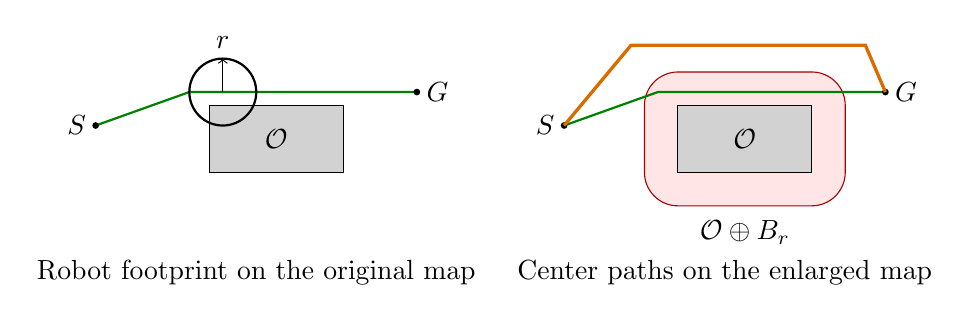
\begin{tikzpicture}[scale=.85]
\foreach \dx in {0,7} {
\begin{scope}[shift={(\dx,0)}]
\ifnum\dx=7
\filldraw[fill=red!10,draw=red!65!black] (2,0.5)--(4,.5) arc(-90:0:.5)--(4.5,2) arc(0:90:.5)--(2,2.5) arc(90:180:.5)--(1.5,1) arc(180:270:.5)--cycle;
\fi
\filldraw[fill=gray!35] (2,1) rectangle (4,2);
\draw[thick,green!50!black] (.3,1.7)--(1.7,2.2)--(5.1,2.2);
\fill (.3,1.7) circle(.05) node[left] {$S$};
\fill (5.1,2.2) circle(.05) node[right] {$G$};
\ifnum\dx=0
\draw[thick] (2.2,2.2) circle(.5);
\draw[->] (2.2,2.2)--(2.2,2.7) node[above] {$r$};
\node at (3,1.5) {$\mathcal O$};
\else
\draw[very thick,orange!85!black] (.3,1.7)--(1.3,2.9)--(4.8,2.9)--(5.1,2.2);
\node at (3,1.5) {$\mathcal O$};
\node at (3,.1) {$\mathcal O\oplus B_r$};
\fi
\end{scope}}
\node at (2.7,-.5) {Robot footprint on the original map};
\node at (9.7,-.5) {Center paths on the enlarged map};
\end{tikzpicture}

\caption{A center path can miss the physical obstacle while the robot
still collides (left). Enlarging the obstacle by the disk radius makes
that same path intersect the forbidden region (right). The orange route
clears the enlarged obstacle.}
\label{fig:l13-inflation}
\end{figure}

A path for the center that stays strictly outside these enlarged obstacles
avoids collision under the model. The footprint has been incorporated
into the map, but the \emph{whole path} must still be checked against the
forbidden region. Checking only its endpoints is insufficient.

A noncircular robot can be enclosed in a disk centered at the chosen
reference point. Enlarging obstacles using that radius is conservative:
it can reject passages the actual robot could traverse in a suitable
orientation. Representing orientation explicitly allows a less conservative
model but generally requires a three-dimensional $(x,y,\theta)$ space.
A further margin can account for bounded positioning or tracking errors.
Map boundaries must also leave room for the robot body.

\section{From a free region to a roadmap}
Let $\mathcal C_{\mathrm{free}}=\mathcal C\setminus\mathcal C_{\mathrm{obs}}$.
Given free start and goal configurations $q_S,q_G$, geometric path planning
seeks a continuous curve in $\mathcal C_{\mathrm{free}}$ joining them.
A timing law subsequently specifies how the robot traverses it, subject
to its motion constraints. Corners or sharp curvature changes may require
slowing, stopping, or smoothing before execution.

A \emph{roadmap} replaces the continuous region with a network of curves
that the robot can follow. Planning then has three parts: access the
network from the start, travel along it, and leave it to reach the goal.
Intersections become graph nodes and connecting curve segments become
graph edges. Selecting a route through that graph is a separate search
problem; constructing the roadmap alone does not select a unique route.

\section{Generalized Voronoi roadmaps}
\subsection{Equidistance to the nearest boundaries}
In a planar free region, a generalized Voronoi roadmap follows points with
two or more distinct nearest obstacle-boundary points. In a corridor,
the centerline is equally far from its two walls. Domain boundaries can
be treated as walls as well when they represent actual limits.

The word \emph{nearest} matters. Being equally far from two distant
obstacles does not put a point on the roadmap if a third obstacle is
closer. For separate obstacle sites, branches satisfy
\[
 d_i(q)=d_j(q)=\min_k d_k(q),\qquad
 d_i(q)=\operatorname{dist}(q,\mathcal O_i).
\]
Boundary features of the same nonconvex obstacle may also generate a
branch. This boundary-based view is often called the medial axis of the
free region.

\begin{figure}[htbp]
\centering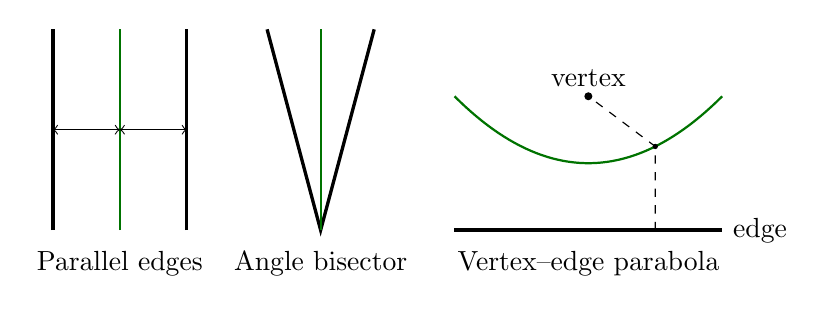
\begin{tikzpicture}[scale=.85]
\draw[very thick] (0,0)--(0,3) (2,0)--(2,3);
\draw[green!45!black,thick] (1,0)--(1,3);
\draw[<->] (0,1.5)--(1,1.5);\draw[<->] (1,1.5)--(2,1.5);
\node at (1,-.5) {Parallel edges};
\begin{scope}[shift={(4,0)}]
\draw[very thick] (-.8,3)--(0,0)--(.8,3);
\draw[green!45!black,thick] (0,0)--(0,3);
\node at (0,-.5) {Angle bisector};
\end{scope}
\begin{scope}[shift={(8,0)}]
\draw[very thick] (-2,0)--(2,0) node[right] {edge};
\fill (0,2) circle(.06) node[above] {vertex};
\draw[green!45!black,thick,domain=-2:2,samples=50] plot (\x,{1+\x*\x/4});
\fill (1,1.25) circle(.04);
\draw[dashed] (1,0)--(1,1.25)--(0,2);
\node at (0,-.5) {Vertex--edge parabola};
\end{scope}
\end{tikzpicture}

\caption{Local equidistance constructions: a midline between parallel
walls, an angle bisector between intersecting supporting lines, and a
parabola between a vertex and an edge. Only portions for which the shown
features are nearest belong to the roadmap.}
\label{fig:l13-features}
\end{figure}

For polygonal obstacles, edge--edge portions can be straight, while a
vertex--edge portion is parabolic. Two vertices generate a perpendicular
bisector. Thus a curved part is not generally a circular arc. At a typical
junction three nearest boundary features meet; special symmetric cases
can produce higher-degree junctions.

Distance requires a metric. Euclidean distance in a position map is
measured in length units. If a plot mixes angles and extensions, a scaling
or weighted metric must be chosen before interpreting equidistance.
Clearance in such a coordinate metric is not directly a physical distance
between the robot body and an obstacle.

\subsection{Sketching and using the roadmap}
\begin{enumerate}
\item Draw the forbidden regions and domain boundaries. Sketch the
midlines or angle bisectors between nearby faces.
\item Follow changes in the closest boundary features. Add vertex--edge
curves where needed, retaining only branches whose generating features
are nearest.
\item Join compatible branches and mark intersections. Check that the
network stays inside the free region.
\item Project $q_S$ and $q_G$ onto the diagram: choose closest points
$r_S$ and $r_G$ anywhere on its branches, and connect them to the start
and goal by straight segments. Check that these access segments are free.
\item Find a network route from $r_S$ to $r_G$ and concatenate
$q_S\to r_S\to r_G\to q_G$.
\end{enumerate}
Writing the diagram as $V$, the projection is
\[
 r_S\in\operatorname*{arg\,min}_{v\in V}\|v-q_S\|,\qquad
 r_G\in\operatorname*{arg\,min}_{v\in V}\|v-q_G\|.
\]
The minimization is over the entire diagram, not just its intersections.
A projection can lie inside a branch; split that graph edge at the
projection when representing the query as a graph. If several points are
equally close, the projection need not be unique. For an approximate or
incomplete diagram, verify the straight access segments explicitly. If a
connector is blocked, a different free access connection is needed.

\begin{figure}[htbp]
\centering% Generated by tools/generate_voronoi_figure.py; do not edit by hand.
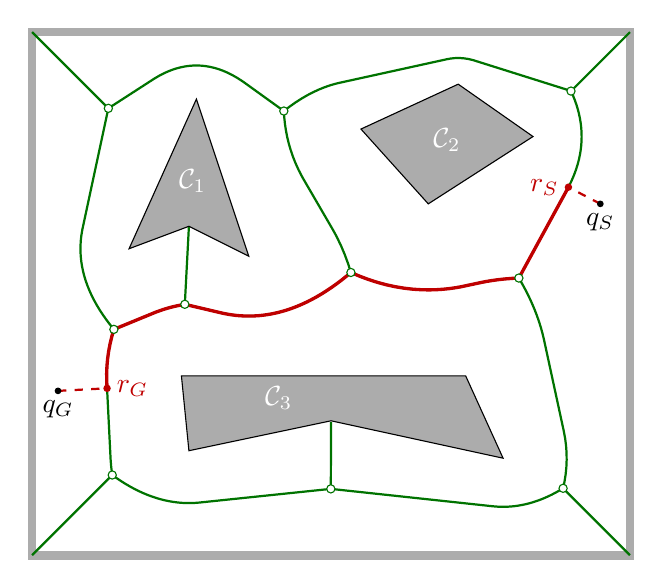
\begin{tikzpicture}[scale=.95]
\draw[line width=3pt,gray!65] (0,0) rectangle (8,7);
\filldraw[fill=gray!65] (1.30000,4.10000)--(2.20000,6.10000)--(2.90000,4.00000)--(2.10000,4.40000)--cycle;
\filldraw[fill=gray!65] (4.40000,5.70000)--(5.70000,6.30000)--(6.70000,5.60000)--(5.30000,4.70000)--cycle;
\filldraw[fill=gray!65] (2.10000,1.40000)--(2.00000,2.40000)--(5.80000,2.40000)--(6.30000,1.30000)--(4.00000,1.80000)--cycle;
\node[white] at (2.15000,5.00000) {$\mathcal C_1$};
\node[white] at (5.55000,5.55000) {$\mathcal C_2$};
\node[white] at (3.30000,2.10000) {$\mathcal C_3$};
\draw[green!45!black,thick] (4.26546,3.78265)--(4.38000,3.73400)--(4.50000,3.68913)--(4.62000,3.65052)--(4.74000,3.61817)--(4.86000,3.59208)--(4.98000,3.57226)--(5.10000,3.55869)--(5.22000,3.55139)--(5.31600,3.55005)--(5.40400,3.55235)--(5.49200,3.55801)--(5.58000,3.56704)--(5.65200,3.57693)--(5.73200,3.59057)--(6.01682,3.65121)--(6.08433,3.66401)--(6.15283,3.67526)--(6.23986,3.68715)--(6.32844,3.69662)--(6.41858,3.70367)--(6.51098,3.70832);
\draw[green!45!black,thick] (4.26546,3.78265)--(4.19600,3.72487)--(4.13200,3.67431)--(4.06800,3.62631)--(3.99600,3.57538)--(3.93200,3.53282)--(3.86800,3.49282)--(3.80400,3.45538)--(3.73200,3.41631)--(3.66800,3.38431)--(3.60400,3.35488)--(3.54000,3.32799)--(3.46800,3.30082)--(3.40400,3.27937)--(3.34000,3.26050)--(3.27600,3.24418)--(3.20400,3.22887)--(3.14800,3.21922)--(3.08400,3.21058)--(3.02800,3.20512)--(2.96400,3.20127)--(2.90800,3.20002)--(2.84400,3.20098)--(2.78000,3.20450)--(2.72400,3.20967)--(2.64400,3.22047)--(2.55600,3.23698)--(2.04527,3.35719);
\draw[green!45!black,thick] (4.26546,3.78265)--(4.22779,3.90101)--(4.18346,4.02177)--(4.13784,4.13065)--(4.08441,4.24322)--(4.05399,4.30152)--(4.02223,4.35862)--(3.61877,5.05246)--(3.56653,5.15298)--(3.52036,5.25552)--(3.48833,5.33750)--(3.46003,5.42073)--(3.43548,5.50521)--(3.41466,5.59093)--(3.39759,5.67790)--(3.38425,5.76611)--(3.37465,5.85557)--(3.36902,5.94119);
\draw[green!45!black,thick] (2.09948,4.39002)--(2.04527,3.35719);
\draw[green!45!black,thick] (1.02294,5.97706)--(0.67520,4.35600)--(0.66302,4.28400)--(0.65482,4.21200)--(0.65061,4.14000)--(0.65039,4.06800)--(0.65354,4.00400)--(0.66085,3.93200)--(0.67070,3.86800)--(0.68369,3.80400)--(0.69984,3.74000)--(0.71914,3.67600)--(0.74159,3.61200)--(0.76719,3.54800)--(0.79594,3.48400)--(0.82784,3.42000)--(0.86289,3.35600)--(0.90609,3.28400)--(0.94784,3.22000)--(0.99274,3.15600)--(1.04079,3.09200)--(1.09678,3.02221);
\draw[green!45!black,thick] (1.02294,5.97706)--(1.63600,6.37329)--(1.70000,6.41112)--(1.76400,6.44440)--(1.82000,6.46979)--(1.87600,6.49169)--(1.93200,6.51011)--(1.98800,6.52504)--(2.04400,6.53649)--(2.10000,6.54445)--(2.15600,6.54893)--(2.21200,6.54993)--(2.26800,6.54744)--(2.32400,6.54147)--(2.38000,6.53201)--(2.44400,6.51693)--(2.50000,6.50001)--(2.55600,6.47960)--(2.61200,6.45571)--(2.67600,6.42413)--(2.74800,6.38317)--(2.82800,6.33091)--(3.36902,5.94119);
\draw[green!45!black,thick] (1.02294,5.97706)--(0.00400,6.99600);
\draw[green!45!black,thick] (7.10238,0.89762)--(7.05200,0.86750)--(7.00400,0.84062)--(6.94800,0.81150)--(6.90000,0.78846)--(6.85200,0.76719)--(6.80400,0.74769)--(6.75600,0.72997)--(6.70000,0.71153)--(6.65200,0.69765)--(6.60400,0.68554)--(6.55600,0.67520)--(6.50000,0.66538)--(6.45200,0.65888)--(6.40400,0.65415)--(6.34800,0.65088)--(6.30000,0.64999)--(6.23600,0.65157)--(6.16400,0.65711)--(3.99701,0.88993);
\draw[green!45!black,thick] (7.10238,0.89762)--(7.12137,0.98800)--(7.13628,1.08400)--(7.14577,1.18000)--(7.14984,1.27600)--(7.14848,1.37200)--(7.14170,1.46800)--(7.12951,1.56400)--(7.11189,1.66000)--(6.84676,2.88400)--(6.82771,2.96400)--(6.80575,3.04400)--(6.78087,3.12400)--(6.75015,3.21200)--(6.71917,3.29200)--(6.68173,3.38000)--(6.64464,3.46000)--(6.60048,3.54800)--(6.55728,3.62800)--(6.51098,3.70832);
\draw[green!45!black,thick] (7.10238,0.89762)--(7.99600,0.00400);
\draw[green!45!black,thick] (3.99701,0.88993)--(3.99993,1.78092);
\draw[green!45!black,thick] (3.99701,0.88993)--(2.23600,0.70660)--(2.18000,0.70228)--(2.12400,0.70020)--(2.06800,0.70036)--(2.01200,0.70276)--(1.95600,0.70740)--(1.89200,0.71545)--(1.83600,0.72489)--(1.77200,0.73842)--(1.71600,0.75266)--(1.66000,0.76914)--(1.60400,0.78786)--(1.54000,0.81199)--(1.48400,0.83551)--(1.42800,0.86127)--(1.36400,0.89346)--(1.30800,0.92402)--(1.24400,0.96169)--(1.18800,0.99705)--(1.13200,1.03465)--(1.07513,1.07513);
\draw[green!45!black,thick] (6.51098,3.70832)--(7.17838,4.93200)--(7.21338,5.00400)--(7.24760,5.08400)--(7.27418,5.15600)--(7.29905,5.23600)--(7.31352,5.29200)--(7.32711,5.35600)--(7.33641,5.41200)--(7.34409,5.47600)--(7.34862,5.54000)--(7.35000,5.59600)--(7.34862,5.66000)--(7.34409,5.72400)--(7.33754,5.78000)--(7.32711,5.84400)--(7.31352,5.90800)--(7.29905,5.96400)--(7.28216,6.02000)--(7.25991,6.08400)--(7.23450,6.14800)--(7.20788,6.20788);
\draw[green!45!black,thick] (3.36902,5.94119)--(3.44400,5.99849)--(3.52400,6.05486)--(3.60400,6.10631)--(3.68400,6.15283)--(3.75600,6.19049)--(3.83600,6.22766)--(3.91600,6.25991)--(3.99600,6.28723)--(4.05200,6.30343)--(4.10800,6.31721)--(5.54800,6.63351)--(5.59600,6.64229)--(5.65200,6.64837)--(5.71600,6.64983)--(5.77200,6.64631)--(5.83600,6.63680)--(5.90000,6.62144)--(7.14000,6.23086)--(7.20788,6.20788);
\draw[green!45!black,thick] (7.20788,6.20788)--(7.99600,6.99600);
\draw[green!45!black,thick] (1.07513,1.07513)--(1.06152,1.18000)--(1.05320,1.28400)--(1.00211,2.30800)--(1.00010,2.42000)--(1.00211,2.49200)--(1.00739,2.57200)--(1.01488,2.64400)--(1.02624,2.72400)--(1.04080,2.80400)--(1.05664,2.87600)--(1.07507,2.94800)--(1.09678,3.02221);
\draw[green!45!black,thick] (1.07513,1.07513)--(0.00400,0.00400);
\draw[green!45!black,thick] (2.04527,3.35719)--(1.94789,3.33879)--(1.86945,3.32056)--(1.79223,3.29908)--(1.70869,3.27169)--(1.62662,3.24037)--(1.09678,3.02221);
\draw[red!75!black,very thick] (7.17371,4.92298)--(6.51098,3.70832)--(6.41858,3.70367)--(6.32844,3.69662)--(6.23986,3.68715)--(6.15283,3.67526)--(6.08433,3.66401)--(6.01682,3.65121)--(5.73200,3.59057)--(5.66000,3.57817)--(5.58000,3.56704)--(5.49200,3.55801)--(5.40400,3.55235)--(5.31600,3.55005)--(5.22000,3.55139)--(5.10000,3.55869)--(4.98000,3.57226)--(4.86000,3.59208)--(4.74000,3.61817)--(4.62000,3.65052)--(4.50000,3.68913)--(4.38000,3.73400)--(4.26546,3.78265)--(4.19600,3.72487)--(4.13200,3.67431)--(4.06800,3.62631)--(4.00400,3.58087)--(3.94000,3.53800)--(3.87600,3.49768)--(3.81200,3.45991)--(3.74000,3.42049)--(3.67600,3.38817)--(3.61200,3.35841)--(3.54800,3.33121)--(3.47600,3.30368)--(3.41200,3.28191)--(3.34800,3.26272)--(3.28400,3.24608)--(3.21200,3.23041)--(3.15600,3.22047)--(3.09200,3.21152)--(3.03600,3.20578)--(2.97200,3.20161)--(2.91600,3.20008)--(2.85200,3.20072)--(2.78800,3.20392)--(2.72400,3.20967)--(2.64400,3.22047)--(2.55600,3.23698)--(2.04527,3.35719)--(1.93999,3.33712)--(1.84616,3.31445)--(1.75407,3.28711)--(1.65629,3.25222)--(1.09678,3.02221)--(1.06864,2.92400)--(1.04579,2.82800)--(1.02755,2.73200)--(1.01299,2.62800)--(1.00435,2.53200)--(1.00032,2.43600)--(1.00067,2.34800)--(1.00578,2.23416);
\filldraw[draw=green!45!black,fill=white] (4.26546,3.78265) circle(.055);
\filldraw[draw=green!45!black,fill=white] (1.02294,5.97706) circle(.055);
\filldraw[draw=green!45!black,fill=white] (7.10238,0.89762) circle(.055);
\filldraw[draw=green!45!black,fill=white] (3.99701,0.88993) circle(.055);
\filldraw[draw=green!45!black,fill=white] (6.51098,3.70832) circle(.055);
\filldraw[draw=green!45!black,fill=white] (3.36902,5.94119) circle(.055);
\filldraw[draw=green!45!black,fill=white] (7.20788,6.20788) circle(.055);
\filldraw[draw=green!45!black,fill=white] (1.07513,1.07513) circle(.055);
\filldraw[draw=green!45!black,fill=white] (2.04527,3.35719) circle(.055);
\filldraw[draw=green!45!black,fill=white] (1.09678,3.02221) circle(.055);
\draw[red!75!black,dashed,thick] (7.60000,4.70000)--(7.17371,4.92298);
\fill (7.60000,4.70000) circle(.045) node[below] {$q_S$};
\fill[red!75!black] (7.17371,4.92298) circle(.05) node[left] {$r_S$};
\draw[red!75!black,dashed,thick] (0.35000,2.20000)--(1.00578,2.23416);
\fill (0.35000,2.20000) circle(.045) node[below] {$q_G$};
\fill[red!75!black] (1.00578,2.23416) circle(.05) node[right] {$r_G$};
\end{tikzpicture}

\caption{A numerically approximated generalized Voronoi roadmap around three polygonal
obstacles and the enclosing walls. Green branches form the network;
the red route joins the projections $r_S$ and $r_G$ inside two branches,
with dashed straight connections from the start and to the goal.
Projections are closest points on the diagram, not nearest intersections.
The branches are computed from densely sampled obstacle boundaries;
straight and curved portions follow the nearest-boundary geometry.}
\label{fig:l13-roadmap}
\end{figure}

Roadmaps based on clearance tend to keep a path away from nearby obstacle
boundaries, which is useful when execution is imperfect. They do not in
general give the shortest route, nor does every branch maximize clearance
globally. Narrow passages still impose small clearance, and the access
connections can approach obstacles more closely than the central route.
Any guarantee also depends on the accuracy of the map and robot model.

\section{Representing a roadmap as a graph}
\label{sec:l13-graphs}
A graph $G=(V,E)$ consists of vertices (nodes) and edges connecting them.
It can represent a road network, communication links, or any specified
relationship. In a roadmap, intersections are nodes and the individual
paths joining adjacent intersections are edges. Start, goal, and their
projections are also inserted as nodes; a projection inside a branch splits
that branch into two edges.

An undirected edge permits travel in both directions. Directed edges
represent allowed directions separately. A simple computer representation
stores node identifiers and edge records $(u,v,w)$, where $w$ is the cost
of traversing the edge. Neighbor lists provide another convenient
representation. The graph drawing is a visualization of these records;
its layout need not preserve physical distances. To execute a route, retain
the geometric path associated with each edge as well.

\begin{figure}[htbp]
\centering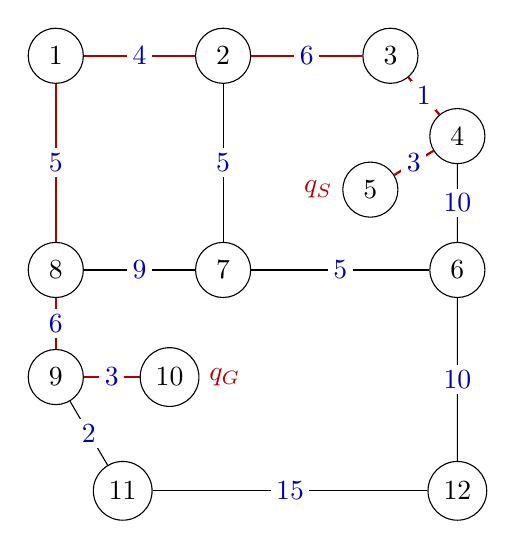
\begin{tikzpicture}[scale=.85,n/.style={circle,draw,fill=white,minimum size=7mm},w/.style={fill=white,inner sep=2pt,text=blue!70!black}]
\foreach \i/\x/\y in {1/0/5,2/2.5/5,3/5/5,4/6/3.8,5/4.7/3,6/6/1.8,7/2.5/1.8,8/0/1.8,9/0/.2,10/1.7/.2,11/1/-1.5,12/6/-1.5}
 \node[n] (n\i) at (\x,\y) {$\i$};
\foreach \a/\b/\c in {1/2/4,1/8/5,2/3/6,2/7/5,3/4/1,4/5/3,4/6/10,6/7/5,6/12/10,7/8/9,8/9/6,9/10/3,9/11/2,11/12/15}
 \draw (n\a)--(n\b) node[midway,w] {$\c$};
\foreach \a/\b in {5/4,4/3,3/2,2/1,1/8,8/9,9/10}
 \draw[red!70!black,thick] (n\a)--(n\b);
\foreach \a/\b/\c in {5/4/3,4/3/1,3/2/6,2/1/4,1/8/5,8/9/6,9/10/3}
 \path (n\a)--(n\b) node[midway,w] {$\c$};
\node[left,red!70!black] at (n5.west) {$q_S$};
\node[right,red!70!black] at (n10.east) {$q_G$};
\end{tikzpicture}

\caption{An undirected weighted roadmap graph. Node 5 is the start and
node 10 is the goal; nodes 4 and 9 represent their roadmap projections.
Weights are assigned example costs, not measurements of this drawing.
The red edges show the minimum-cost route.}
\label{fig:l13-weighted}
\end{figure}

For a sequence of adjacent nodes $v_0,\ldots,v_m$, the path cost is
\begin{equation}
 J=\sum_{k=0}^{m-1}w(v_k,v_{k+1}).
 \label{eq:l13-pathcost}
\end{equation}
If weights are physical lengths, minimizing $J$ finds a shortest route
on the graph. Other choices can represent time or penalties. A graph
route is not necessarily the shortest path in the continuous free space.
For the assigned weights in Figure~\ref{fig:l13-weighted}, the visually
plausible route $5,4,6,7,8,9,10$ costs
$3+10+5+9+6+3=36$. A systematic search finds a route of cost 28.

\section{Dijkstra's algorithm}
\label{sec:l13-dijkstra}
Dijkstra's algorithm applies to nonnegative edge costs. It maintains a
best known cumulative cost $g(v)$ from the start and a predecessor $p(v)$
for each reached node. An \emph{open} node has a tentative cost and awaits
selection. A \emph{settled} node has been selected with minimum open cost;
its cost is then final.

\subsection{Selection and relaxation}
\begin{enumerate}
\item Set $g(q_S)=0$ and all other costs to infinity. Put the start in
the open set; initially there are no predecessors or settled nodes.
\item Select the node $u$ with smallest $g(u)$ among \emph{all} open
nodes. Remove it from the open set and settle it.
\item If $u=q_G$, stop successfully. Otherwise consider each unsettled
neighbor $v$ and form the candidate $g(u)+w(u,v)$.
\item If this candidate is smaller than $g(v)$, replace $g(v)$ and set
$p(v)=u$. Insert $v$ into the open set or update its priority there.
This operation is called \emph{relaxation}.
\item Repeat. If the open set becomes empty before the goal is selected,
there is no route from start to goal in this graph.
\end{enumerate}
The selection is global over the frontier, not restricted to neighbors
of the most recently expanded node. Nonnegative weights ensure that an
alternative path through a node with higher tentative cost cannot later
improve the node just settled. Zero-weight edges are allowed; equal-cost
choices can be resolved consistently without changing the optimal cost.

\subsection{A complete trace}
For the graph in Figure~\ref{fig:l13-weighted}, the selection order and
successful updates are:
\begin{center}
\begin{tabular}{crl}
\toprule
Selected node & Final cost & New or improved tentative costs\\
\midrule
5 & 0 & $g(4)=3$\\
4 & 3 & $g(3)=4,\quad g(6)=13$\\
3 & 4 & $g(2)=10$\\
2 & 10 & $g(1)=14,\quad g(7)=15$\\
6 & 13 & $g(12)=23$; candidate 18 for node 7 rejected\\
1 & 14 & $g(8)=19$\\
7 & 15 & No improvement: candidate 24 for node 8 rejected\\
8 & 19 & $g(9)=25$\\
12 & 23 & $g(11)=38$\\
9 & 25 & $g(10)=28,\quad g(11):38\to27$\\
11 & 27 & No improvement\\
10 & 28 & Goal selected: stop\\
\bottomrule
\end{tabular}
\end{center}
Node 11 illustrates a predecessor change: it is initially reached from
12 at cost 38, then improved through 9 to cost 27. Node 12 must be selected
before 9 because $23<25$, even though the drawing places node 9 nearer
the goal. Dijkstra uses accumulated cost rather than visual direction.

\begin{figure}[htbp]
\centering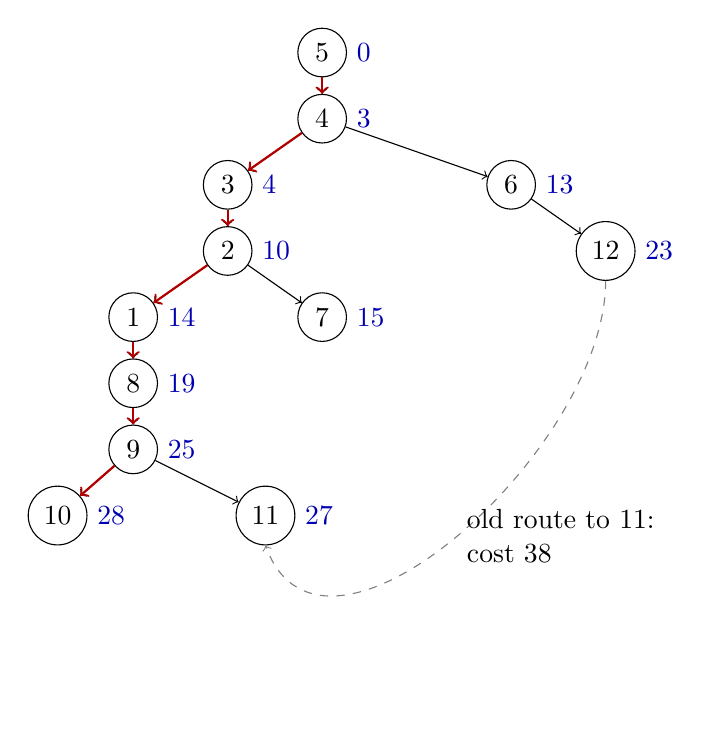
\begin{tikzpicture}[x=1.2cm,y=.6cm,n/.style={circle,draw,fill=white,minimum size=6mm}]
\foreach \i/\x/\y/\g in {5/0/0/0,4/0/-1.4/3,3/-1/-2.8/4,6/2/-2.8/13,2/-1/-4.2/10,1/-2/-5.6/14,7/0/-5.6/15,8/-2/-7/19,9/-2/-8.4/25,10/-2.8/-9.8/28,11/-.6/-9.8/27,12/3/-4.2/23} {
\node[n] (n\i) at (\x,\y) {$\i$};
\node[right,blue!70!black] at (n\i.east) {$\g$};}
\foreach \a/\b in {5/4,4/3,4/6,3/2,2/1,2/7,1/8,8/9,9/10,9/11,6/12}
 \draw[->] (n\a)--(n\b);
\foreach \a/\b in {5/4,4/3,3/2,2/1,1/8,8/9,9/10}
 \draw[->,red!70!black,thick] (n\a)--(n\b);
\draw[->,dashed,gray] (n12) to[out=-90,in=-70] node[right,align=left,text=black] {old route to 11:\\cost 38} (n11.south);
\end{tikzpicture}

\caption{Predecessor tree at termination, with cumulative costs in blue.
The dashed link is the superseded predecessor of node 11, first reached
through 12 at cost 38. The final red chain reconstructs the solution.
Only one final predecessor is retained for each non-root node.}
\label{fig:l13-tree}
\end{figure}

During a hand execution one may draw duplicate candidate occurrences of
a graph node and cross out the more expensive ones. In a cost/predecessor
implementation these occurrences correspond to comparisons against the
same stored $g(v)$. A better candidate changes that node's predecessor;
it does not create a distinct physical location.

Once the goal is selected, follow predecessors backward:
\[
 10\leftarrow9\leftarrow8\leftarrow1\leftarrow2\leftarrow3
 \leftarrow4\leftarrow5.
\]
Reverse this list to obtain the forward route. Its cost is
\[
 3+1+6+4+5+6+3=28.
\]
Each consecutive pair identifies an original roadmap edge. Executing the
route follows those stored geometric curves, rather than new straight
segments between node positions.

\subsection{Why discovering the goal is not enough}
Node 10 is first discovered at cost 28 while node 11 remains open at 27.
The algorithm must select 11 before declaring 10 optimal. In the original
graph this produces no further improvement, but the rule is essential.

To see why, modify the graph by replacing $w(9,11)=2$ with 1 and adding
an undirected edge $(11,10)$ of weight 1. Node 9 now discovers node 10 at
28 and improves node 11 to 26. Expanding 11 improves the goal to
$26+1=27$, giving
\[
 5\to4\to3\to2\to1\to8\to9\to11\to10.
\]
Stopping at first discovery would return the inferior cost 28. The correct
stopping event is selecting the goal as the minimum-cost open node.

\section{A brief introduction to A*}
A* prioritizes an open node by
\begin{equation}
 f(v)=g(v)+h(v),
 \label{eq:l13-astar}
\end{equation}
where $h(v)$ estimates the remaining cost to the goal. This can concentrate
the search on promising regions and reduce the number of expanded nodes.
Setting $h=0$ recovers Dijkstra's selection rule. The heuristic changes
the exploration order, not the definition of the accumulated path cost.

When nodes have Cartesian positions and edge weights are lengths of
physical paths, straight-line distance to the goal is a useful heuristic.
It does not overestimate the remaining route length. It also satisfies
the consistency condition $h(u)\le w(u,v)+h(v)$ for every edge, so an
A* graph search that settles nodes need not reopen them. With a merely
admissible but inconsistent heuristic, improved nodes may need reopening
to retain optimality.

Arbitrary example weights do not automatically support an unscaled
Cartesian-distance heuristic. Its units and lower-bound property must
match the chosen cost. A* does not permanently discard a branch merely
because it initially points away from the goal; obstacles can require
such detours. A useful heuristic can save work, but faster execution is
not guaranteed for every problem.

\section{Exact cell decomposition by a sweep line}
\label{sec:l13-sweep}
Another way to construct a planning graph is to partition the free region
into simple cells. For polygonal obstacles and a polygonal outer boundary,
choose a fixed sweep direction. At each vertex event, introduce parallel
cuts through free space. A full-cut construction extends each event line
through every free interval of the domain; it can subdivide more than
the minimal vertical decomposition, but remains an exact decomposition.
Obstacle interiors are excluded from the cells.

Between consecutive event coordinates the boundaries are straight and
do not change order. Each connected free cell is a triangle or trapezoid
(including rectangular cases) and is convex. Convexity means the segment
between any two points in the cell stays in the cell. A nonconvex region
does not have this property for every pair of points.

\begin{figure}[htbp]
\centering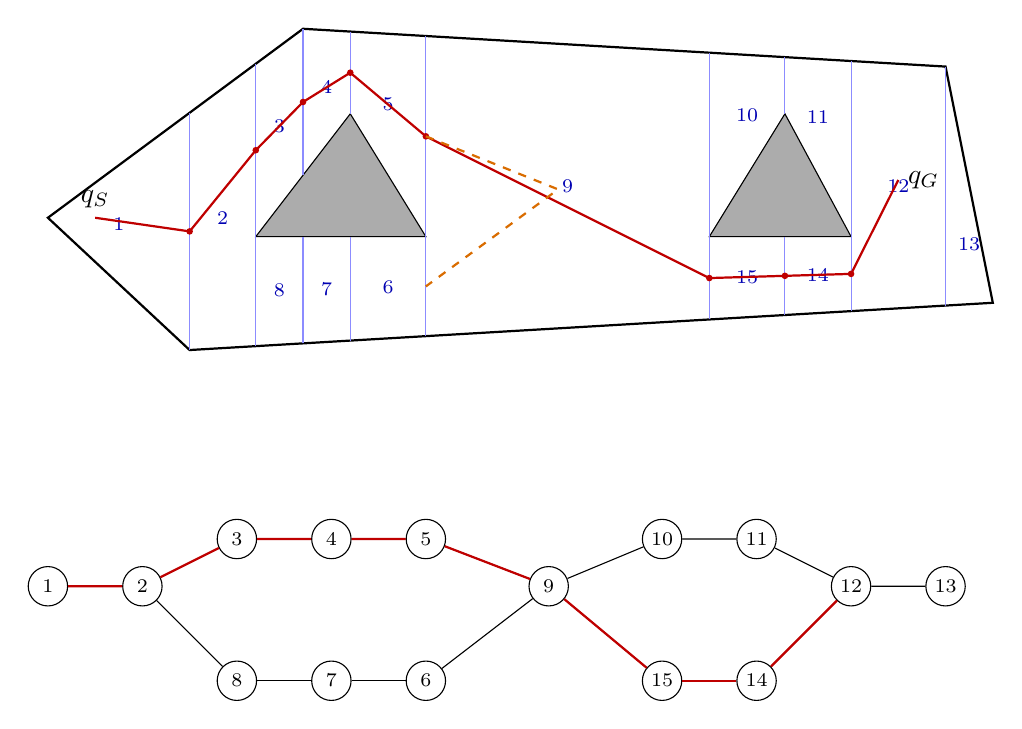
\begin{tikzpicture}[scale=1.2]
\draw[thick] (0.0000,1.4000)--(2.7000,3.4000)--(9.5000,3.0000)--(10.0000,0.5000)--(1.5000,0.0000)--cycle;
\filldraw[fill=gray!65] (2.2000,1.2000)--(3.2000,2.5000)--(4.0000,1.2000)--cycle;
\filldraw[fill=gray!65] (7.0000,1.2000)--(7.8000,2.5000)--(8.5000,1.2000)--cycle;
\draw[thin,blue!45] (1.5000,0.0000)--(1.5000,2.5111);
\draw[thin,blue!45] (2.2000,0.0412)--(2.2000,1.2000);
\draw[thin,blue!45] (2.2000,1.2000)--(2.2000,3.0296);
\draw[thin,blue!45] (2.7000,0.0706)--(2.7000,1.2000);
\draw[thin,blue!45] (2.7000,1.8500)--(2.7000,3.4000);
\draw[thin,blue!45] (3.2000,0.1000)--(3.2000,1.2000);
\draw[thin,blue!45] (3.2000,2.5000)--(3.2000,3.3706);
\draw[thin,blue!45] (4.0000,0.1471)--(4.0000,1.2000);
\draw[thin,blue!45] (4.0000,1.2000)--(4.0000,3.3235);
\draw[thin,blue!45] (7.0000,0.3235)--(7.0000,1.2000);
\draw[thin,blue!45] (7.0000,1.2000)--(7.0000,3.1471);
\draw[thin,blue!45] (7.8000,0.3706)--(7.8000,1.2000);
\draw[thin,blue!45] (7.8000,2.5000)--(7.8000,3.1000);
\draw[thin,blue!45] (8.5000,0.4118)--(8.5000,1.2000);
\draw[thin,blue!45] (8.5000,1.2000)--(8.5000,3.0588);
\draw[thin,blue!45] (9.5000,0.4706)--(9.5000,3.0000);
\node[blue!70!black,font=\scriptsize] at (0.7500,1.3278) {1};
\node[blue!70!black,font=\scriptsize] at (1.8500,1.3955) {2};
\node[blue!70!black,font=\scriptsize] at (2.4500,0.6279) {8};
\node[blue!70!black,font=\scriptsize] at (2.4500,2.3699) {3};
\node[blue!70!black,font=\scriptsize] at (2.9500,0.6426) {7};
\node[blue!70!black,font=\scriptsize] at (2.9500,2.7801) {4};
\node[blue!70!black,font=\scriptsize] at (3.6000,0.6618) {6};
\node[blue!70!black,font=\scriptsize] at (3.6000,2.5985) {5};
\node[blue!70!black,font=\scriptsize] at (5.5000,1.7353) {9};
\node[blue!70!black,font=\scriptsize] at (7.4000,0.7735) {15};
\node[blue!70!black,font=\scriptsize] at (7.4000,2.4868) {10};
\node[blue!70!black,font=\scriptsize] at (8.1500,0.7956) {14};
\node[blue!70!black,font=\scriptsize] at (8.1500,2.4647) {11};
\node[blue!70!black,font=\scriptsize] at (9.0000,1.7353) {12};
\node[blue!70!black,font=\scriptsize] at (9.7500,1.1176) {13};
\draw[red!75!black,thick] (0.5000,1.4000)--(1.5000,1.2556)--(2.2000,2.1148)--(2.7000,2.6250)--(3.2000,2.9353)--(4.0000,2.2618)--(7.0000,0.7618)--(7.8000,0.7853)--(8.5000,0.8059)--(9.0000,1.8000);
\fill[red!75!black] (1.5000,1.2556) circle(.035);
\fill[red!75!black] (2.2000,2.1148) circle(.035);
\fill[red!75!black] (2.7000,2.6250) circle(.035);
\fill[red!75!black] (3.2000,2.9353) circle(.035);
\fill[red!75!black] (4.0000,2.2618) circle(.035);
\fill[red!75!black] (7.0000,0.7618) circle(.035);
\fill[red!75!black] (7.8000,0.7853) circle(.035);
\fill[red!75!black] (8.5000,0.8059) circle(.035);
\node[above] at (0.5000,1.4000) {$q_S$};
\node[right] at (9.0000,1.8000) {$q_G$};
\draw[orange!85!black,thick,dashed] (4.0000,2.2618)--(5.4,1.7)--(4.0000,0.6735);
\begin{scope}[yshift=-3.5cm,n/.style={circle,draw,fill=white,minimum size=5mm,inner sep=1pt,font=\scriptsize}]
\node[n] (n1) at (0.0000,1.0000) {1};
\node[n] (n2) at (1.0000,1.0000) {2};
\node[n] (n3) at (2.0000,1.5000) {3};
\node[n] (n4) at (3.0000,1.5000) {4};
\node[n] (n5) at (4.0000,1.5000) {5};
\node[n] (n9) at (5.3000,1.0000) {9};
\node[n] (n10) at (6.5000,1.5000) {10};
\node[n] (n11) at (7.5000,1.5000) {11};
\node[n] (n12) at (8.5000,1.0000) {12};
\node[n] (n13) at (9.5000,1.0000) {13};
\node[n] (n8) at (2.0000,0.0000) {8};
\node[n] (n7) at (3.0000,0.0000) {7};
\node[n] (n6) at (4.0000,0.0000) {6};
\node[n] (n15) at (6.5000,0.0000) {15};
\node[n] (n14) at (7.5000,0.0000) {14};
\draw (n1)--(n2);
\draw (n2)--(n3);
\draw (n2)--(n8);
\draw (n3)--(n4);
\draw (n4)--(n5);
\draw (n8)--(n7);
\draw (n7)--(n6);
\draw (n5)--(n9);
\draw (n6)--(n9);
\draw (n9)--(n10);
\draw (n10)--(n11);
\draw (n11)--(n12);
\draw (n9)--(n15);
\draw (n15)--(n14);
\draw (n14)--(n12);
\draw (n12)--(n13);
\draw[red!75!black,thick] (n1)--(n2);
\draw[red!75!black,thick] (n2)--(n3);
\draw[red!75!black,thick] (n3)--(n4);
\draw[red!75!black,thick] (n4)--(n5);
\draw[red!75!black,thick] (n5)--(n9);
\draw[red!75!black,thick] (n9)--(n15);
\draw[red!75!black,thick] (n15)--(n14);
\draw[red!75!black,thick] (n14)--(n12);
\end{scope}
\end{tikzpicture}

\caption{Full vertical cuts through polygon vertices partition the free
region into 15 convex cells. The connectivity graph records free portals
between cells. The red route uses the sequence
$1,2,3,4,5,9,15,14,12$; the orange detour illustrates passing through an
interior point when entering and leaving cell 9 on the same side.
The geometry preserves the two-obstacle layout and cell numbering.}
\label{fig:l13-cells}
\end{figure}

\subsection{Connectivity and geometric reconstruction}
Represent each cell by a graph node. Connect cells that share a
traversable boundary interval, called a \emph{portal}. Mere contact at
an obstacle vertex does not create a usable passage when obstacle contact
counts as collision. Identify the cells containing $q_S$ and $q_G$, then
search their connectivity graph.

The result is initially a sequence of cells, not yet a geometric path.
Choose a point in the relative interior of each free portal, such as its
midpoint. Connect the start, successive portal points, and the goal with
segments inside the corresponding cells. Convexity keeps those segments
inside cell closures, but obstacle boundaries are forbidden. If two portal
points lie on the same supporting line and their direct connection runs
along an obstacle, insert a point strictly inside the cell and connect
through it instead. This occurs for the sequence $5,9,6$ in the figure.

The complete procedure is therefore:
\begin{enumerate}
\item Decompose the free region with parallel sweep cuts.
\item Number the cells and construct the portal-adjacency graph.
\item Locate the start and goal cells and run graph search.
\item Select free portal points along the returned sequence.
\item Construct and check the geometric segments, adding interior
waypoints where necessary.
\end{enumerate}
An unweighted adjacency graph can minimize the number of cell transitions.
That objective is not necessarily geometric path length. To optimize a
length cost, the graph representation and weights must account for the
actual connectors being used. Similarly, exact decomposition describes
the represented geometry faithfully; it does not imply exact knowledge
of a real environment or automatic dynamic feasibility of the path.

\section{Approximate cell decomposition}
\label{sec:l13-approximate}
Exact decomposition follows obstacle geometry. An alternative is to cover
configuration space with simple cells and refine the cells whose status is
uncertain. In two dimensions, a square can be divided into four equal
squares; repeating this operation produces a \emph{quadtree}. Small cells
resolve obstacle boundaries while large cells can represent open regions.

Consider a bounded two-dimensional configuration space. Enclose it in a
square if necessary, treating the region outside the permitted domain as
forbidden. Classify each cell by its interior:
\begin{itemize}
\item \textbf{Empty:} its interior contains only free configurations.
\item \textbf{Occupied:} its interior is entirely forbidden.
\item \textbf{Mixed:} it contains both free and forbidden configurations.
\end{itemize}
Obstacle contact still counts as collision. Calling a cell empty does
not make every point on its boundary free: shared boundaries must be
checked when constructing transitions.

\subsection{Refinement guided by a connectivity graph}
The following procedure uses an \emph{optimistic} graph: mixed cells are
temporarily allowed, but a route through them is only a candidate.
\begin{enumerate}
\item Split the initial square into four cells and classify them.
\item Create a graph node for each nonoccupied cell. Connect cells that
share a boundary segment of positive length through which a transition
might be possible. Do not connect cells merely because they share a corner.
For two empty cells, require a free portion of their common boundary.
\item Locate the cells containing $q_S$ and $q_G$ and search the graph
between them. First check that the start and goal themselves are free.
Prefer a route using only empty cells: search that subgraph first, and
use the optimistic graph if no such route is available yet.
\item If the candidate route includes mixed cells, subdivide mixed cells
into four, update the graph, and search again. A simple implementation
refines all mixed cells at each iteration.
\item Once the route uses only empty cells, choose a free crossing point
on each shared boundary and construct a continuous path through those
points. Validate the resulting path before accepting it.
\end{enumerate}
A conservative alternative excludes mixed cells from the graph. In that
version, an unsuccessful search can trigger further subdivision: a passage
may exist inside cells that have not yet been resolved.

Figure~\ref{fig:l13-quadtree} illustrates three successive resolutions.
The initial graph is small but cannot certify a route. Refinement reveals
occupied cells inside the larger obstacle and creates smaller cells around
both obstacle boundaries. A large empty square remains in the lower-left
region throughout: there is no need to subdivide every cell uniformly.

\begin{figure}[p]
\centering% Generated by tools/generate_sampling_figures.py
\begin{tikzpicture}[scale=0.65,line cap=round,line join=round,
 every node/.style={font=\footnotesize},>=Stealth]
\begin{scope}[yshift=-0.0cm]
\node[anchor=west,font=\small\bfseries] at (0,8.6) {Iteration 1: 4 cells};
\fill[white] (0.0000,0.0000) rectangle (4.0000,4.0000);
\fill[black!12] (4.0000,0.0000) rectangle (8.0000,4.0000);
\fill[black!12] (0.0000,4.0000) rectangle (4.0000,8.0000);
\fill[black!12] (4.0000,4.0000) rectangle (8.0000,8.0000);
\fill[black!85] (1.8000,5.2000) -- (2.7000,7.0000) -- (3.7000,5.2000) -- cycle;
\fill[black!85] (4.0000,2.0000) -- (6.0000,2.0000) -- (6.0000,2.5000) -- (6.8000,2.5000) -- (6.8000,6.7000) -- (5.0000,6.7000) -- (5.0000,6.0000) -- (4.0000,6.0000) -- cycle;
\draw[black!45,thin] (0.0000,0.0000) rectangle (4.0000,4.0000);
\draw[black!45,thin] (4.0000,0.0000) rectangle (8.0000,4.0000);
\draw[black!45,thin] (0.0000,4.0000) rectangle (4.0000,8.0000);
\draw[black!45,thin] (4.0000,4.0000) rectangle (8.0000,8.0000);
\draw[thick] (0,0) rectangle (8,8);
\fill[robotframe] (0.4000,7.3000) circle (2pt);
\node[fill=white,inner sep=1pt,above right] at (0.4000,7.3000) {$q_S$};
\fill[robotframe] (7.5000,1.3000) circle (2pt);
\node[fill=white,inner sep=1pt,above right] at (7.5000,1.3000) {$q_G$};
\begin{scope}[xshift=9.5cm]
\draw[black!20] (0,0) rectangle (8,8);
\draw[black!50] (6.0000,2.0000) -- (2.0000,2.0000);
\draw[black!50] (2.0000,6.0000) -- (2.0000,2.0000);
\draw[black!50] (6.0000,6.0000) -- (6.0000,2.0000);
\draw[black!50] (6.0000,6.0000) -- (2.0000,6.0000);
\draw[robotframe,very thick] (2.0000,6.0000) -- (2.0000,2.0000) -- (6.0000,2.0000);
\draw[fill=white] (2.0000,2.0000) circle (3pt);
\draw[fill=black!40] (6.0000,2.0000) circle (3pt);
\draw[fill=black!40] (2.0000,6.0000) circle (3pt);
\draw[fill=black!40] (6.0000,6.0000) circle (3pt);
\node[above left,fill=white,inner sep=1pt] at (2.0000,6.0000) {$C_S$};
\node[above left,fill=white,inner sep=1pt] at (6.0000,2.0000) {$C_G$};
\end{scope}
\end{scope}
\begin{scope}[yshift=-9.4cm]
\node[anchor=west,font=\small\bfseries] at (0,8.6) {Iteration 2: 13 cells};
\fill[white] (0.0000,0.0000) rectangle (4.0000,4.0000);
\fill[white] (4.0000,0.0000) rectangle (6.0000,2.0000);
\fill[white] (6.0000,0.0000) rectangle (8.0000,2.0000);
\fill[black!65] (4.0000,2.0000) rectangle (6.0000,4.0000);
\fill[black!12] (6.0000,2.0000) rectangle (8.0000,4.0000);
\fill[black!12] (0.0000,4.0000) rectangle (2.0000,6.0000);
\fill[black!12] (2.0000,4.0000) rectangle (4.0000,6.0000);
\fill[white] (0.0000,6.0000) rectangle (2.0000,8.0000);
\fill[black!12] (2.0000,6.0000) rectangle (4.0000,8.0000);
\fill[black!65] (4.0000,4.0000) rectangle (6.0000,6.0000);
\fill[black!12] (6.0000,4.0000) rectangle (8.0000,6.0000);
\fill[black!12] (4.0000,6.0000) rectangle (6.0000,8.0000);
\fill[black!12] (6.0000,6.0000) rectangle (8.0000,8.0000);
\fill[black!85] (1.8000,5.2000) -- (2.7000,7.0000) -- (3.7000,5.2000) -- cycle;
\fill[black!85] (4.0000,2.0000) -- (6.0000,2.0000) -- (6.0000,2.5000) -- (6.8000,2.5000) -- (6.8000,6.7000) -- (5.0000,6.7000) -- (5.0000,6.0000) -- (4.0000,6.0000) -- cycle;
\draw[black!45,thin] (0.0000,0.0000) rectangle (4.0000,4.0000);
\draw[black!45,thin] (4.0000,0.0000) rectangle (6.0000,2.0000);
\draw[black!45,thin] (6.0000,0.0000) rectangle (8.0000,2.0000);
\draw[black!45,thin] (4.0000,2.0000) rectangle (6.0000,4.0000);
\draw[black!45,thin] (6.0000,2.0000) rectangle (8.0000,4.0000);
\draw[black!45,thin] (0.0000,4.0000) rectangle (2.0000,6.0000);
\draw[black!45,thin] (2.0000,4.0000) rectangle (4.0000,6.0000);
\draw[black!45,thin] (0.0000,6.0000) rectangle (2.0000,8.0000);
\draw[black!45,thin] (2.0000,6.0000) rectangle (4.0000,8.0000);
\draw[black!45,thin] (4.0000,4.0000) rectangle (6.0000,6.0000);
\draw[black!45,thin] (6.0000,4.0000) rectangle (8.0000,6.0000);
\draw[black!45,thin] (4.0000,6.0000) rectangle (6.0000,8.0000);
\draw[black!45,thin] (6.0000,6.0000) rectangle (8.0000,8.0000);
\draw[thick] (0,0) rectangle (8,8);
\fill[robotframe] (0.4000,7.3000) circle (2pt);
\node[fill=white,inner sep=1pt,above right] at (0.4000,7.3000) {$q_S$};
\fill[robotframe] (7.5000,1.3000) circle (2pt);
\node[fill=white,inner sep=1pt,above right] at (7.5000,1.3000) {$q_G$};
\begin{scope}[xshift=9.5cm]
\draw[black!20] (0,0) rectangle (8,8);
\draw[black!50] (5.0000,1.0000) -- (2.0000,2.0000);
\draw[black!50] (7.0000,1.0000) -- (5.0000,1.0000);
\draw[black!50] (7.0000,3.0000) -- (7.0000,1.0000);
\draw[black!50] (1.0000,5.0000) -- (2.0000,2.0000);
\draw[black!50] (3.0000,5.0000) -- (2.0000,2.0000);
\draw[black!50] (3.0000,5.0000) -- (1.0000,5.0000);
\draw[black!50] (1.0000,7.0000) -- (1.0000,5.0000);
\draw[black!50] (3.0000,7.0000) -- (3.0000,5.0000);
\draw[black!50] (3.0000,7.0000) -- (1.0000,7.0000);
\draw[black!50] (7.0000,5.0000) -- (7.0000,3.0000);
\draw[black!50] (5.0000,7.0000) -- (3.0000,7.0000);
\draw[black!50] (7.0000,7.0000) -- (7.0000,5.0000);
\draw[black!50] (7.0000,7.0000) -- (5.0000,7.0000);
\draw[robotframe,very thick] (1.0000,7.0000) -- (1.0000,5.0000) -- (2.0000,2.0000) -- (5.0000,1.0000) -- (7.0000,1.0000);
\draw[fill=white] (2.0000,2.0000) circle (3pt);
\draw[fill=white] (5.0000,1.0000) circle (3pt);
\draw[fill=white] (7.0000,1.0000) circle (3pt);
\draw[fill=black!40] (7.0000,3.0000) circle (3pt);
\draw[fill=black!40] (1.0000,5.0000) circle (3pt);
\draw[fill=black!40] (3.0000,5.0000) circle (3pt);
\draw[fill=white] (1.0000,7.0000) circle (3pt);
\draw[fill=black!40] (3.0000,7.0000) circle (3pt);
\draw[fill=black!40] (7.0000,5.0000) circle (3pt);
\draw[fill=black!40] (5.0000,7.0000) circle (3pt);
\draw[fill=black!40] (7.0000,7.0000) circle (3pt);
\node[above left,fill=white,inner sep=1pt] at (1.0000,7.0000) {$C_S$};
\node[above left,fill=white,inner sep=1pt] at (7.0000,1.0000) {$C_G$};
\end{scope}
\end{scope}
\begin{scope}[yshift=-18.8cm]
\node[anchor=west,font=\small\bfseries] at (0,8.6) {Iteration 3: 34 cells};
\fill[white] (0.0000,0.0000) rectangle (4.0000,4.0000);
\fill[white] (4.0000,0.0000) rectangle (6.0000,2.0000);
\fill[white] (6.0000,0.0000) rectangle (8.0000,2.0000);
\fill[black!65] (4.0000,2.0000) rectangle (6.0000,4.0000);
\fill[black!12] (6.0000,2.0000) rectangle (7.0000,3.0000);
\fill[white] (7.0000,2.0000) rectangle (8.0000,3.0000);
\fill[black!12] (6.0000,3.0000) rectangle (7.0000,4.0000);
\fill[white] (7.0000,3.0000) rectangle (8.0000,4.0000);
\fill[white] (0.0000,4.0000) rectangle (1.0000,5.0000);
\fill[white] (1.0000,4.0000) rectangle (2.0000,5.0000);
\fill[white] (0.0000,5.0000) rectangle (1.0000,6.0000);
\fill[black!12] (1.0000,5.0000) rectangle (2.0000,6.0000);
\fill[white] (2.0000,4.0000) rectangle (3.0000,5.0000);
\fill[white] (3.0000,4.0000) rectangle (4.0000,5.0000);
\fill[black!12] (2.0000,5.0000) rectangle (3.0000,6.0000);
\fill[black!12] (3.0000,5.0000) rectangle (4.0000,6.0000);
\fill[white] (0.0000,6.0000) rectangle (2.0000,8.0000);
\fill[black!12] (2.0000,6.0000) rectangle (3.0000,7.0000);
\fill[black!12] (3.0000,6.0000) rectangle (4.0000,7.0000);
\fill[white] (2.0000,7.0000) rectangle (3.0000,8.0000);
\fill[white] (3.0000,7.0000) rectangle (4.0000,8.0000);
\fill[black!65] (4.0000,4.0000) rectangle (6.0000,6.0000);
\fill[black!12] (6.0000,4.0000) rectangle (7.0000,5.0000);
\fill[white] (7.0000,4.0000) rectangle (8.0000,5.0000);
\fill[black!12] (6.0000,5.0000) rectangle (7.0000,6.0000);
\fill[white] (7.0000,5.0000) rectangle (8.0000,6.0000);
\fill[white] (4.0000,6.0000) rectangle (5.0000,7.0000);
\fill[black!12] (5.0000,6.0000) rectangle (6.0000,7.0000);
\fill[white] (4.0000,7.0000) rectangle (5.0000,8.0000);
\fill[white] (5.0000,7.0000) rectangle (6.0000,8.0000);
\fill[black!12] (6.0000,6.0000) rectangle (7.0000,7.0000);
\fill[white] (7.0000,6.0000) rectangle (8.0000,7.0000);
\fill[white] (6.0000,7.0000) rectangle (7.0000,8.0000);
\fill[white] (7.0000,7.0000) rectangle (8.0000,8.0000);
\fill[black!85] (1.8000,5.2000) -- (2.7000,7.0000) -- (3.7000,5.2000) -- cycle;
\fill[black!85] (4.0000,2.0000) -- (6.0000,2.0000) -- (6.0000,2.5000) -- (6.8000,2.5000) -- (6.8000,6.7000) -- (5.0000,6.7000) -- (5.0000,6.0000) -- (4.0000,6.0000) -- cycle;
\draw[black!45,thin] (0.0000,0.0000) rectangle (4.0000,4.0000);
\draw[black!45,thin] (4.0000,0.0000) rectangle (6.0000,2.0000);
\draw[black!45,thin] (6.0000,0.0000) rectangle (8.0000,2.0000);
\draw[black!45,thin] (4.0000,2.0000) rectangle (6.0000,4.0000);
\draw[black!45,thin] (6.0000,2.0000) rectangle (7.0000,3.0000);
\draw[black!45,thin] (7.0000,2.0000) rectangle (8.0000,3.0000);
\draw[black!45,thin] (6.0000,3.0000) rectangle (7.0000,4.0000);
\draw[black!45,thin] (7.0000,3.0000) rectangle (8.0000,4.0000);
\draw[black!45,thin] (0.0000,4.0000) rectangle (1.0000,5.0000);
\draw[black!45,thin] (1.0000,4.0000) rectangle (2.0000,5.0000);
\draw[black!45,thin] (0.0000,5.0000) rectangle (1.0000,6.0000);
\draw[black!45,thin] (1.0000,5.0000) rectangle (2.0000,6.0000);
\draw[black!45,thin] (2.0000,4.0000) rectangle (3.0000,5.0000);
\draw[black!45,thin] (3.0000,4.0000) rectangle (4.0000,5.0000);
\draw[black!45,thin] (2.0000,5.0000) rectangle (3.0000,6.0000);
\draw[black!45,thin] (3.0000,5.0000) rectangle (4.0000,6.0000);
\draw[black!45,thin] (0.0000,6.0000) rectangle (2.0000,8.0000);
\draw[black!45,thin] (2.0000,6.0000) rectangle (3.0000,7.0000);
\draw[black!45,thin] (3.0000,6.0000) rectangle (4.0000,7.0000);
\draw[black!45,thin] (2.0000,7.0000) rectangle (3.0000,8.0000);
\draw[black!45,thin] (3.0000,7.0000) rectangle (4.0000,8.0000);
\draw[black!45,thin] (4.0000,4.0000) rectangle (6.0000,6.0000);
\draw[black!45,thin] (6.0000,4.0000) rectangle (7.0000,5.0000);
\draw[black!45,thin] (7.0000,4.0000) rectangle (8.0000,5.0000);
\draw[black!45,thin] (6.0000,5.0000) rectangle (7.0000,6.0000);
\draw[black!45,thin] (7.0000,5.0000) rectangle (8.0000,6.0000);
\draw[black!45,thin] (4.0000,6.0000) rectangle (5.0000,7.0000);
\draw[black!45,thin] (5.0000,6.0000) rectangle (6.0000,7.0000);
\draw[black!45,thin] (4.0000,7.0000) rectangle (5.0000,8.0000);
\draw[black!45,thin] (5.0000,7.0000) rectangle (6.0000,8.0000);
\draw[black!45,thin] (6.0000,6.0000) rectangle (7.0000,7.0000);
\draw[black!45,thin] (7.0000,6.0000) rectangle (8.0000,7.0000);
\draw[black!45,thin] (6.0000,7.0000) rectangle (7.0000,8.0000);
\draw[black!45,thin] (7.0000,7.0000) rectangle (8.0000,8.0000);
\draw[thick] (0,0) rectangle (8,8);
\draw[robotframe,very thick] (0.4000,7.3000) -- (1.0000,7.0000) -- (0.5000,6.0000) -- (0.5000,5.5000) -- (0.5000,5.0000) -- (0.5000,4.5000) -- (0.5000,4.0000) -- (2.0000,2.0000) -- (4.0000,1.0000) -- (5.0000,1.0000) -- (6.0000,1.0000) -- (7.0000,1.0000) -- (7.5000,1.3000);
\fill[robotframe] (0.4000,7.3000) circle (2pt);
\node[fill=white,inner sep=1pt,above right] at (0.4000,7.3000) {$q_S$};
\fill[robotframe] (7.5000,1.3000) circle (2pt);
\node[fill=white,inner sep=1pt,above right] at (7.5000,1.3000) {$q_G$};
\begin{scope}[xshift=9.5cm]
\draw[black!20] (0,0) rectangle (8,8);
\draw[black!50] (5.0000,1.0000) -- (2.0000,2.0000);
\draw[black!50] (7.0000,1.0000) -- (5.0000,1.0000);
\draw[black!50] (6.5000,2.5000) -- (7.0000,1.0000);
\draw[black!50] (7.5000,2.5000) -- (7.0000,1.0000);
\draw[black!50] (7.5000,2.5000) -- (6.5000,2.5000);
\draw[black!50] (6.5000,3.5000) -- (6.5000,2.5000);
\draw[black!50] (7.5000,3.5000) -- (7.5000,2.5000);
\draw[black!50] (7.5000,3.5000) -- (6.5000,3.5000);
\draw[black!50] (0.5000,4.5000) -- (2.0000,2.0000);
\draw[black!50] (1.5000,4.5000) -- (2.0000,2.0000);
\draw[black!50] (1.5000,4.5000) -- (0.5000,4.5000);
\draw[black!50] (0.5000,5.5000) -- (0.5000,4.5000);
\draw[black!50] (1.5000,5.5000) -- (1.5000,4.5000);
\draw[black!50] (1.5000,5.5000) -- (0.5000,5.5000);
\draw[black!50] (2.5000,4.5000) -- (2.0000,2.0000);
\draw[black!50] (2.5000,4.5000) -- (1.5000,4.5000);
\draw[black!50] (3.5000,4.5000) -- (2.0000,2.0000);
\draw[black!50] (3.5000,4.5000) -- (2.5000,4.5000);
\draw[black!50] (2.5000,5.5000) -- (1.5000,5.5000);
\draw[black!50] (2.5000,5.5000) -- (2.5000,4.5000);
\draw[black!50] (3.5000,5.5000) -- (3.5000,4.5000);
\draw[black!50] (3.5000,5.5000) -- (2.5000,5.5000);
\draw[black!50] (1.0000,7.0000) -- (0.5000,5.5000);
\draw[black!50] (1.0000,7.0000) -- (1.5000,5.5000);
\draw[black!50] (2.5000,6.5000) -- (2.5000,5.5000);
\draw[black!50] (2.5000,6.5000) -- (1.0000,7.0000);
\draw[black!50] (3.5000,6.5000) -- (3.5000,5.5000);
\draw[black!50] (3.5000,6.5000) -- (2.5000,6.5000);
\draw[black!50] (2.5000,7.5000) -- (1.0000,7.0000);
\draw[black!50] (2.5000,7.5000) -- (2.5000,6.5000);
\draw[black!50] (3.5000,7.5000) -- (3.5000,6.5000);
\draw[black!50] (3.5000,7.5000) -- (2.5000,7.5000);
\draw[black!50] (6.5000,4.5000) -- (6.5000,3.5000);
\draw[black!50] (7.5000,4.5000) -- (7.5000,3.5000);
\draw[black!50] (7.5000,4.5000) -- (6.5000,4.5000);
\draw[black!50] (6.5000,5.5000) -- (6.5000,4.5000);
\draw[black!50] (7.5000,5.5000) -- (7.5000,4.5000);
\draw[black!50] (7.5000,5.5000) -- (6.5000,5.5000);
\draw[black!50] (4.5000,6.5000) -- (3.5000,6.5000);
\draw[black!50] (5.5000,6.5000) -- (4.5000,6.5000);
\draw[black!50] (4.5000,7.5000) -- (3.5000,7.5000);
\draw[black!50] (4.5000,7.5000) -- (4.5000,6.5000);
\draw[black!50] (5.5000,7.5000) -- (5.5000,6.5000);
\draw[black!50] (5.5000,7.5000) -- (4.5000,7.5000);
\draw[black!50] (6.5000,6.5000) -- (6.5000,5.5000);
\draw[black!50] (6.5000,6.5000) -- (5.5000,6.5000);
\draw[black!50] (7.5000,6.5000) -- (7.5000,5.5000);
\draw[black!50] (7.5000,6.5000) -- (6.5000,6.5000);
\draw[black!50] (6.5000,7.5000) -- (5.5000,7.5000);
\draw[black!50] (6.5000,7.5000) -- (6.5000,6.5000);
\draw[black!50] (7.5000,7.5000) -- (7.5000,6.5000);
\draw[black!50] (7.5000,7.5000) -- (6.5000,7.5000);
\draw[robotframe,very thick] (1.0000,7.0000) -- (0.5000,5.5000) -- (0.5000,4.5000) -- (2.0000,2.0000) -- (5.0000,1.0000) -- (7.0000,1.0000);
\draw[fill=white] (2.0000,2.0000) circle (3pt);
\draw[fill=white] (5.0000,1.0000) circle (3pt);
\draw[fill=white] (7.0000,1.0000) circle (3pt);
\draw[fill=black!40] (6.5000,2.5000) circle (3pt);
\draw[fill=white] (7.5000,2.5000) circle (3pt);
\draw[fill=black!40] (6.5000,3.5000) circle (3pt);
\draw[fill=white] (7.5000,3.5000) circle (3pt);
\draw[fill=white] (0.5000,4.5000) circle (3pt);
\draw[fill=white] (1.5000,4.5000) circle (3pt);
\draw[fill=white] (0.5000,5.5000) circle (3pt);
\draw[fill=black!40] (1.5000,5.5000) circle (3pt);
\draw[fill=white] (2.5000,4.5000) circle (3pt);
\draw[fill=white] (3.5000,4.5000) circle (3pt);
\draw[fill=black!40] (2.5000,5.5000) circle (3pt);
\draw[fill=black!40] (3.5000,5.5000) circle (3pt);
\draw[fill=white] (1.0000,7.0000) circle (3pt);
\draw[fill=black!40] (2.5000,6.5000) circle (3pt);
\draw[fill=black!40] (3.5000,6.5000) circle (3pt);
\draw[fill=white] (2.5000,7.5000) circle (3pt);
\draw[fill=white] (3.5000,7.5000) circle (3pt);
\draw[fill=black!40] (6.5000,4.5000) circle (3pt);
\draw[fill=white] (7.5000,4.5000) circle (3pt);
\draw[fill=black!40] (6.5000,5.5000) circle (3pt);
\draw[fill=white] (7.5000,5.5000) circle (3pt);
\draw[fill=white] (4.5000,6.5000) circle (3pt);
\draw[fill=black!40] (5.5000,6.5000) circle (3pt);
\draw[fill=white] (4.5000,7.5000) circle (3pt);
\draw[fill=white] (5.5000,7.5000) circle (3pt);
\draw[fill=black!40] (6.5000,6.5000) circle (3pt);
\draw[fill=white] (7.5000,6.5000) circle (3pt);
\draw[fill=white] (6.5000,7.5000) circle (3pt);
\draw[fill=white] (7.5000,7.5000) circle (3pt);
\node[above left,fill=white,inner sep=1pt] at (1.0000,7.0000) {$C_S$};
\node[above left,fill=white,inner sep=1pt] at (7.0000,1.0000) {$C_G$};
\end{scope}
\end{scope}
\end{tikzpicture}

\caption{Approximate decomposition and its connectivity graphs, using the
same obstacles at all three iterations. White cells/nodes are empty,
gray ones are mixed, and black cells are occupied and excluded from the
graphs. Red graph routes in iterations 1 and 2 are provisional because
they visit mixed cells. The third route uses only empty cells; the map
shows a validated geometric realization through free portals and cell
interiors. Graph edges describe adjacency, not executable straight paths
between cell centers when mixed cells are involved.}
\label{fig:l13-quadtree}
\end{figure}

\subsection{From cells to a path}
For adjacent empty cells, the free part of their shared side is a
\emph{portal}. Its midpoint is a convenient crossing point when the
whole portal is free. Join consecutive crossings through the cell interior,
inserting an interior waypoint if a direct connection would follow a
forbidden boundary. Square cells are convex, so interior waypoints make
this construction particularly simple. Include connections from $q_S$
and to $q_G$.

Refinement requires a stopping rule, such as a maximum depth or minimum
cell width. Failure to obtain a certified route at that resolution does
not generally prove that no continuous path exists. A narrow passage can
remain hidden in mixed cells. Conversely, a graph disconnected even when
all mixed cells are allowed can certify separation if that graph includes
every possible transition under the chosen domain assumptions.

A shortest route on the cell graph minimizes its assigned graph cost.
It need not be the shortest geometric path. Refining only mixed cells
does not by itself establish convergence to the continuous shortest path.
After constructing a feasible path, one can try collision-checked
\emph{shortcuts}: replace a subpath by a straight segment only when the
entire replacement is free. This can reduce length without certifying
global optimality.

\section{Probabilistic roadmaps}
\label{sec:l13-prm}
Cell decompositions construct a representation by partitioning space.
A \emph{probabilistic roadmap} (PRM) instead samples configurations and
connects nearby samples with feasible local paths. Different samples can
produce different graphs, so adding samples can reveal connections that
were absent in an earlier attempt.

For a point moving in a planar free region, a local path can be a straight
segment. A simple construction is:
\begin{enumerate}
\item Sample a batch of $N$ configurations in the domain.
\item Reject configurations in collision. Retain the free samples as nodes.
\item For pairs closer than a connection radius $d$, test the complete
straight segment between them. Add an edge only if that segment is free.
Assign a cost, such as its Euclidean length.
\item Insert $q_S$ and $q_G$ and connect them by the same local test.
Search the graph using Dijkstra or another suitable graph-search method.
\item If no route exists in the current graph, add more samples and
connections, subject to a computation budget, and search again.
\end{enumerate}
In a fixed environment the roadmap can be reused for different start--goal
queries. Only the query configurations and their connections need to be
inserted again, provided the robot model and collision geometry are unchanged.

\begin{figure}[htbp]
\centering% Generated by tools/generate_sampling_figures.py
\begin{tikzpicture}[scale=1.35,line cap=round,line join=round,
 every node/.style={font=\footnotesize},>=Stealth]
\draw[thick] (0.0000,0.0000) -- (10.0000,0.0000) -- (9.3000,3.7000) -- (3.0000,3.3000) -- cycle;
\fill[black!85] (2.5000,1.0000) -- (4.0000,2.5000) -- (4.5000,0.8000) -- cycle;
\fill[black!85] (6.0000,1.2000) -- (7.8000,1.2000) -- (8.0000,2.7000) -- (6.1000,2.7000) -- cycle;
\draw[black!40] (4.1000,0.4500) -- (2.1000,0.6500);
\draw[black!40] (6.0000,3.0000) -- (4.9000,1.8000);
\draw[black!40] (8.3000,2.1000) -- (8.5000,0.6000);
\draw[black!40] (2.0000,1.5000) -- (3.0000,2.9500);
\draw[black!40] (2.0000,1.5000) -- (2.1000,0.6500);
\draw[black!40] (4.6000,2.9000) -- (3.0000,2.9500);
\draw[black!40] (4.6000,2.9000) -- (4.9000,1.8000);
\draw[black!40] (4.6000,2.9000) -- (6.0000,3.0000);
\draw[black!40] (5.7000,0.5000) -- (4.1000,0.4500);
\draw[black!40] (5.7000,0.5000) -- (4.9000,1.8000);
\draw[black!40] (7.0000,0.5000) -- (8.5000,0.6000);
\draw[black!40] (7.0000,0.5000) -- (5.7000,0.5000);
\draw[black!40] (8.7000,3.1000) -- (8.3000,2.1000);
\draw[black!40] (2.8000,2.0000) -- (3.0000,2.9500);
\draw[black!40] (2.8000,2.0000) -- (2.1000,0.6500);
\draw[black!40] (2.8000,2.0000) -- (2.0000,1.5000);
\draw[black!40] (2.8000,2.0000) -- (4.6000,2.9000);
\draw[black!40] (3.0000,0.4000) -- (2.1000,0.6500);
\draw[black!40] (3.0000,0.4000) -- (4.1000,0.4500);
\draw[black!40] (3.0000,0.4000) -- (2.0000,1.5000);
\draw[black!40] (5.8000,1.6000) -- (4.1000,0.4500);
\draw[black!40] (5.8000,1.6000) -- (4.9000,1.8000);
\draw[black!40] (5.8000,1.6000) -- (6.0000,3.0000);
\draw[black!40] (5.8000,1.6000) -- (4.6000,2.9000);
\draw[black!40] (5.8000,1.6000) -- (5.7000,0.5000);
\draw[black!40] (8.6000,1.3000) -- (8.5000,0.6000);
\draw[black!40] (8.6000,1.3000) -- (8.3000,2.1000);
\draw[black!40] (8.6000,1.3000) -- (7.0000,0.5000);
\draw[black!40] (8.6000,1.3000) -- (8.7000,3.1000);
\draw[black!40] (7.4000,3.2000) -- (6.0000,3.0000);
\draw[black!40] (7.4000,3.2000) -- (8.7000,3.1000);
\draw[red!75!black,dashed,thick] (2.8000,2.0000) -- (4.9000,1.8000);
\draw[robotframe,very thick] (3.0000,2.9500) -- (4.6000,2.9000) -- (4.9000,1.8000) -- (5.7000,0.5000) -- (7.0000,0.5000) -- (8.5000,0.6000);
\draw[black,fill=white,thick] (3.0000,2.9500) circle (2.5pt);
\draw[black,fill=white,thick] (8.5000,0.6000) circle (2.5pt);
\draw[sensorframe,fill=white,thick] (2.1000,0.6500) circle (2.5pt);
\draw[sensorframe,fill=white,thick] (4.1000,0.4500) circle (2.5pt);
\draw[sensorframe,fill=white,thick] (4.9000,1.8000) circle (2.5pt);
\draw[sensorframe,fill=white,thick] (6.0000,3.0000) circle (2.5pt);
\draw[sensorframe,fill=white,thick] (8.3000,2.1000) circle (2.5pt);
\draw[orange!90!black,fill=white,thick] (2.0000,1.5000) circle (2.5pt);
\draw[orange!90!black,fill=white,thick] (4.6000,2.9000) circle (2.5pt);
\draw[orange!90!black,fill=white,thick] (5.7000,0.5000) circle (2.5pt);
\draw[orange!90!black,fill=white,thick] (7.0000,0.5000) circle (2.5pt);
\draw[orange!90!black,fill=white,thick] (8.7000,3.1000) circle (2.5pt);
\draw[green!50!black,fill=white,thick] (2.8000,2.0000) circle (2.5pt);
\draw[green!50!black,fill=white,thick] (3.0000,0.4000) circle (2.5pt);
\draw[green!50!black,fill=white,thick] (5.8000,1.6000) circle (2.5pt);
\draw[green!50!black,fill=white,thick] (8.6000,1.3000) circle (2.5pt);
\draw[green!50!black,fill=white,thick] (7.4000,3.2000) circle (2.5pt);
\node[red,font=\large] at (3.7000,1.5000) {$\times$};
\node[red,font=\large] at (6.8000,1.8000) {$\times$};
\node[above] at (3.0000,2.9500) {$q_S$};
\node[below] at (8.5000,0.6000) {$q_G$};
\node[anchor=west] at (0,-.5) {Samples: \textcolor{sensorframe}{batch 1}, \textcolor{orange!90!black}{batch 2}, \textcolor{green!50!black}{batch 3}};
\end{tikzpicture}

\caption{A sampled roadmap in a polygonal domain. Sample colors distinguish
three batches; red crosses mark rejected configurations inside obstacles.
The dashed red candidate edge has free endpoints but crosses the triangular
obstacle, so it is rejected. The highlighted route consists entirely of
validated edges. Coordinates are illustrative.}
\label{fig:l13-prm}
\end{figure}

\subsection{Checking nodes is not enough}
Two free configurations can lie on opposite sides of an obstacle. Thus
node validity and edge validity are separate tests. If an attempted edge
is blocked, remove that edge, not its otherwise valid endpoints: those
nodes may still connect to other neighbors. The same distinction applies
when an edge is a curved robot motion rather than a straight line.

The radius $d$ controls the candidate connections. A small radius reduces
the number of attempted edges but can leave the graph disconnected.
A larger radius offers more connections and requires more collision tests.
For configurations involving angles or mixed units, the distance used to
select neighbors must be defined appropriately; it is not automatically
ordinary distance between unscaled coordinate entries.

\subsection{What randomness does and does not guarantee}
An unsuccessful finite run means that the current samples and connections
did not produce a route. It does not establish that the planning problem
is impossible. Biasing samples toward the goal or a likely corridor can
help, but excluding other regions can remove the only feasible detour.

Two different properties must be distinguished:
\begin{itemize}
\item \textbf{Probabilistic completeness:} for a feasible problem satisfying
the method's assumptions, the probability of finding a solution approaches
one as the number of samples grows.
\item \textbf{Asymptotic optimality:} under the relevant assumptions, the
best solution cost converges to the optimal cost as sampling continues.
\end{itemize}
Neither property means that a finite run must succeed or return the
continuous optimum. Dijkstra finds the optimum on the constructed graph;
that alone proves neither property for the sampling procedure. Guarantees
depend on the sampling distribution, local planner, connection rule, and
geometry. PRM* is a roadmap variant designed for asymptotic optimality.

\section{Growing search trees}
\label{sec:l13-trees}
A roadmap may connect many pairs of samples. A tree instead gives each
new node one parent and grows outward from an initial configuration.
Once a node has a valid connection to the goal, its parent chain recovers
a path to the root. There is no need to run Dijkstra merely to recover
the unique path already stored in that tree.

\subsection{A local branching construction}
A useful geometric construction starts at $q_S$, proposes a few points
at distance $d$ from it, and retains the collision-free connecting segments.
Repeat from the new nodes, drawing successive generations in different
colors. Reject candidates whose motions hit an obstacle or leave the domain.
An unsuccessful extension does not necessarily make its parent useless:
another direction from the same parent may be valid.

If every accepted edge has length $d$, a node at depth $k$ has path
length $kd$. Expanding by increasing depth then agrees with increasing
path cost. If lengths differ, use accumulated edge costs instead. A
priority based on cost plus a suitable heuristic can guide this kind of
search, but it defines a different expansion policy from standard RRT.
Figure~\ref{fig:l13-local-tree} shows the local construction.

\begin{figure}[htbp]
\centering% Generated by tools/generate_sampling_figures.py
\begin{tikzpicture}[scale=1.35,line cap=round,line join=round,
 every node/.style={font=\footnotesize},>=Stealth]
\draw[thick] (0,0) rectangle (9,4.5);
\fill[black!85] (1.4000,2.1000) -- (2.0000,3.4000) -- (2.7000,2.1000) -- cycle;
\fill[black!85] (5.0000,1.1000) -- (6.2000,3.4000) -- (7.5000,1.1000) -- cycle;
\draw[robotframe,thick] (0.4500,4.0000) -- (0.7578,3.1543);
\fill[robotframe] (0.7578,3.1543) circle (1.5pt);
\draw[robotframe,thick] (0.4500,4.0000) -- (1.3363,3.8437);
\fill[robotframe] (1.3363,3.8437) circle (1.5pt);
\draw[red!65,dashed] (0.4500,4.0000) -- (0.7578,4.8457);
\node[red!65] at (0.7578,4.8457) {$\times$};
\draw[red!65,dashed] (0.4500,4.0000) -- (-0.2394,4.5785);
\node[red!65] at (-0.2394,4.5785) {$\times$};
\draw[red!65,dashed] (0.4500,4.0000) -- (-0.3957,3.6922);
\node[red!65] at (-0.3957,3.6922) {$\times$};
\draw[green!50!black,thick] (0.7578,3.1543) -- (0.6856,2.2572);
\fill[green!50!black] (0.6856,2.2572) circle (1.5pt);
\draw[green!50!black,thick] (0.7578,3.1543) -- (1.4525,2.5821);
\fill[green!50!black] (1.4525,2.5821) circle (1.5pt);
\draw[green!50!black,thick] (1.3363,3.8437) -- (2.1403,3.4392);
\fill[green!50!black] (2.1403,3.4392) circle (1.5pt);
\draw[green!50!black,thick] (1.3363,3.8437) -- (2.2191,4.0187);
\fill[green!50!black] (2.2191,4.0187) circle (1.5pt);
\draw[sensorframe,thick] (0.6856,2.2572) -- (0.3079,1.4403);
\fill[sensorframe] (0.3079,1.4403) circle (1.5pt);
\draw[sensorframe,thick] (0.6856,2.2572) -- (1.0527,1.4354);
\fill[sensorframe] (1.0527,1.4354) circle (1.5pt);
\draw[red!65,dashed] (1.4525,2.5821) -- (1.8809,1.7906);
\node[red!65] at (1.8809,1.7906) {$\times$};
\draw[red!65,dashed] (1.4525,2.5821) -- (2.2899,2.2523);
\node[red!65] at (2.2899,2.2523) {$\times$};
\draw[sensorframe,thick] (2.1403,3.4392) -- (2.5872,2.6580);
\fill[sensorframe] (2.5872,2.6580) circle (1.5pt);
\draw[sensorframe,thick] (2.1403,3.4392) -- (3.0383,3.3796);
\fill[sensorframe] (3.0383,3.3796) circle (1.5pt);
\draw[sensorframe,thick] (2.2191,4.0187) -- (3.1072,3.8725);
\fill[sensorframe] (3.1072,3.8725) circle (1.5pt);
\draw[sensorframe,thick] (2.2191,4.0187) -- (2.9844,4.4924);
\fill[sensorframe] (2.9844,4.4924) circle (1.5pt);
\draw[red!65,dashed] (0.3079,1.4403) -- (-0.3794,0.8592);
\node[red!65] at (-0.3794,0.8592) {$\times$};
\draw[violet,thick] (0.3079,1.4403) -- (0.2592,0.5416);
\fill[violet] (0.2592,0.5416) circle (1.5pt);
\draw[violet,thick] (1.0527,1.4354) -- (1.1359,0.5393);
\fill[violet] (1.1359,0.5393) circle (1.5pt);
\draw[violet,thick] (1.0527,1.4354) -- (1.8082,0.9464);
\fill[violet] (1.8082,0.9464) circle (1.5pt);
\draw[red!65,dashed] (2.5872,2.6580) -- (2.6343,1.7592);
\node[red!65] at (2.6343,1.7592) {$\times$};
\draw[violet,thick] (2.5872,2.6580) -- (3.3944,2.2599);
\fill[violet] (3.3944,2.2599) circle (1.5pt);
\draw[violet,thick] (3.0383,3.3796) -- (3.7601,2.8420);
\fill[violet] (3.7601,2.8420) circle (1.5pt);
\draw[violet,thick] (3.0383,3.3796) -- (3.8414,3.7858);
\fill[violet] (3.8414,3.7858) circle (1.5pt);
\draw[violet,thick] (3.1072,3.8725) -- (3.9048,3.4556);
\fill[violet] (3.9048,3.4556) circle (1.5pt);
\draw[violet,thick] (3.1072,3.8725) -- (3.9952,4.0189);
\fill[violet] (3.9952,4.0189) circle (1.5pt);
\draw[red!65,dashed] (2.9844,4.4924) -- (3.8695,4.6557);
\node[red!65] at (3.8695,4.6557) {$\times$};
\draw[red!65,dashed] (2.9844,4.4924) -- (3.4638,5.2541);
\node[red!65] at (3.4638,5.2541) {$\times$};
\draw[red!65,dashed] (0.2592,0.5416) -- (-0.0473,-0.3046);
\node[red!65] at (-0.0473,-0.3046) {$\times$};
\draw[red!65,dashed] (0.2592,0.5416) -- (0.5175,-0.3205);
\node[red!65] at (0.5175,-0.3205) {$\times$};
\draw[red!65,dashed] (1.1359,0.5393) -- (0.8432,-0.3118);
\node[red!65] at (0.8432,-0.3118) {$\times$};
\draw[red!65,dashed] (1.1359,0.5393) -- (1.6799,-0.1777);
\node[red!65] at (1.6799,-0.1777) {$\times$};
\draw[orange!85!black,thick] (1.8082,0.9464) -- (2.3190,0.2054);
\fill[orange!85!black] (2.3190,0.2054) circle (1.5pt);
\draw[orange!85!black,thick] (1.8082,0.9464) -- (2.6906,0.7693);
\fill[orange!85!black] (2.6906,0.7693) circle (1.5pt);
\draw[orange!85!black,thick] (3.3944,2.2599) -- (3.8608,1.4902);
\fill[orange!85!black] (3.8608,1.4902) circle (1.5pt);
\draw[orange!85!black,thick] (3.3944,2.2599) -- (4.2883,2.3643);
\fill[orange!85!black] (4.2883,2.3643) circle (1.5pt);
\draw[orange!85!black,thick] (3.7601,2.8420) -- (4.1807,2.0463);
\fill[orange!85!black] (4.1807,2.0463) circle (1.5pt);
\draw[orange!85!black,thick] (3.7601,2.8420) -- (4.6591,2.7990);
\fill[orange!85!black] (4.6591,2.7990) circle (1.5pt);
\draw[orange!85!black,thick] (3.8414,3.7858) -- (4.7385,3.7133);
\fill[orange!85!black] (4.7385,3.7133) circle (1.5pt);
\draw[red!65,dashed] (3.8414,3.7858) -- (4.3256,4.5444);
\node[red!65] at (4.3256,4.5444) {$\times$};
\draw[orange!85!black,thick] (3.9048,3.4556) -- (4.5191,2.7978);
\fill[orange!85!black] (4.5191,2.7978) circle (1.5pt);
\draw[orange!85!black,thick] (3.9048,3.4556) -- (4.8014,3.5334);
\fill[orange!85!black] (4.8014,3.5334) circle (1.5pt);
\draw[orange!85!black,thick] (3.9952,4.0189) -- (4.8154,3.6484);
\fill[orange!85!black] (4.8154,3.6484) circle (1.5pt);
\draw[orange!85!black,thick] (3.9952,4.0189) -- (4.7579,4.4967);
\fill[orange!85!black] (4.7579,4.4967) circle (1.5pt);
\fill (0.4500,4.0000) circle (2pt) node[below right] {$q_S$};
\fill (4.4,.65) circle (2pt) node[right] {$q_G$};
\node[anchor=west] at (0,-.7) {Generations: \textcolor{robotframe}{1}, \textcolor{green!50!black}{2}, \textcolor{sensorframe}{3}, \textcolor{violet}{4}, \textcolor{orange!85!black}{5}};
\end{tikzpicture}

\caption{Local branching from $q_S$ with equal-length candidate steps.
Colors identify successive generations. Dashed red extensions and crosses
mark rejected candidates; the existing free parent nodes remain valid.
The tree has not yet reached $q_G$. This generation-by-generation
construction illustrates tree growth; it does not use the standard RRT
node-selection rule.}
\label{fig:l13-local-tree}
\end{figure}

\subsection{Rapidly exploring random trees}
An \emph{RRT}, or \emph{rapidly exploring random tree}, selects where to
expand using a sample from the configuration space. For a planar geometric
problem, one iteration is:
\begin{enumerate}
\item Sample a target configuration $q_{\mathrm{rand}}$.
\item Find the tree vertex $q_{\mathrm{near}}$ closest to that target.
\item Steer from $q_{\mathrm{near}}$ toward $q_{\mathrm{rand}}$ by at most
a chosen step length $d$, obtaining a candidate $q_{\mathrm{new}}$.
\item If the complete extension is free, add $q_{\mathrm{new}}$ with
parent $q_{\mathrm{near}}$; otherwise reject the extension.
\end{enumerate}
In Euclidean coordinates, for a nonzero separation, the steering step is
\[
 q_{\mathrm{new}}=q_{\mathrm{near}}+
 \min\!\left(1,\frac{d}{\|q_{\mathrm{rand}}-q_{\mathrm{near}}\|}\right)
 (q_{\mathrm{rand}}-q_{\mathrm{near}}).
\]
Figure~\ref{fig:l13-rrt-step} separates the random target from the new
vertex actually added. The target need not become a tree node.

\begin{figure}[htbp]
\centering% Generated by tools/generate_sampling_figures.py
\begin{tikzpicture}[scale=1.35,line cap=round,line join=round,
 every node/.style={font=\footnotesize},>=Stealth]
\draw[black!20] (0,0) rectangle (8,4);
\draw[thick] (0.5000,0.4000) -- (1.3000,1.3000);
\draw[thick] (1.3000,1.3000) -- (1.0000,2.2000);
\draw[thick] (1.3000,1.3000) -- (2.5000,1.8000);
\draw[thick] (2.5000,1.8000) -- (3.5000,1.1000);
\draw[thick] (2.5000,1.8000) -- (3.0000,3.0000);
\fill (0.5000,0.4000) circle (2pt);
\fill (1.3000,1.3000) circle (2pt);
\fill (1.0000,2.2000) circle (2pt);
\fill (2.5000,1.8000) circle (2pt);
\fill (3.5000,1.1000) circle (2pt);
\fill (3.0000,3.0000) circle (2pt);
\draw[sensorframe,dashed] (4.7868,1.6515) -- (7.0000,2.6000);
\draw[sensorframe,very thick,->] (3.5000,1.1000) -- (4.7868,1.6515) node[midway,above left] {$d$};
\fill[sensorframe] (4.7868,1.6515) circle (2.5pt) node[below right] {$q_{\mathrm{new}}$};
\draw[sensorframe,thick] (7.0000,2.6000) circle (3pt) node[above] {$q_{\mathrm{rand}}$};
\node[below] at (3.5000,1.1000) {$q_{\mathrm{near}}$};
\node[below right] at (0.5000,0.4000) {$q_S$};
\end{tikzpicture}

\caption{One RRT extension. A global random target selects its nearest
existing tree vertex. Only the short, validated extension to
$q_{\mathrm{new}}$ is inserted; the dashed remainder is not a tree edge.}
\label{fig:l13-rrt-step}
\end{figure}

Each vertex has a region of targets for which it is the nearest vertex:
its Voronoi region relative to the tree vertices. Under uniform sampling,
vertices with larger such regions are selected more frequently. This
helps exploration spread into uncovered space. RRT therefore does not
simply expand every leaf once per generation.

The goal may be represented by a small goal region, or the planner may
attempt a checked connection to $q_G$ from a nearby vertex. Occasionally
sampling the goal itself is another useful bias. Closeness alone is not
a valid final edge: that connection must satisfy collision and motion
constraints. Basic RRT seeks a feasible path and is not generally
asymptotically optimal; RRT* adds a cost-aware parent choice and rewiring.

\subsection{Bidirectional growth}
Two trees can be rooted at $q_S$ and $q_G$ and grown toward one another.
When vertices in different trees can be joined by a valid local path,
concatenate the start-tree path, the connecting motion, and the goal-tree
path. In a reversible geometric problem the goal-tree edges can be
traversed in reverse order.

\begin{figure}[htbp]
\centering% Generated by tools/generate_sampling_figures.py
\begin{tikzpicture}[scale=1.35,line cap=round,line join=round,
 every node/.style={font=\footnotesize},>=Stealth]
\draw[thick] (0,0) rectangle (9,4.8);
\fill[black!85] (2.6000,0.9000) -- (6.1000,0.9000) -- (6.4000,2.7000) -- (3.0000,2.8000) -- cycle;
\draw[sensorframe,thick] (0.6000,3.5000) -- (1.5000,3.7000);
\draw[sensorframe,thick] (1.5000,3.7000) -- (2.4000,4.0000);
\draw[sensorframe,thick] (2.4000,4.0000) -- (3.5000,4.1000);
\draw[sensorframe,thick] (0.6000,3.5000) -- (1.1000,2.4000);
\draw[sensorframe,thick] (1.1000,2.4000) -- (0.5000,1.5000);
\draw[sensorframe,thick] (1.1000,2.4000) -- (1.8000,1.7000);
\draw[sensorframe,thick] (1.8000,1.7000) -- (2.3000,1.2000);
\fill[sensorframe] (0.6000,3.5000) circle (2pt);
\fill[sensorframe] (1.5000,3.7000) circle (2pt);
\fill[sensorframe] (2.4000,4.0000) circle (2pt);
\fill[sensorframe] (3.5000,4.1000) circle (2pt);
\fill[sensorframe] (1.1000,2.4000) circle (2pt);
\fill[sensorframe] (0.5000,1.5000) circle (2pt);
\fill[sensorframe] (1.8000,1.7000) circle (2pt);
\fill[sensorframe] (2.3000,1.2000) circle (2pt);
\draw[green!50!black,thick] (8.5000,3.4000) -- (7.8000,3.9000);
\draw[green!50!black,thick] (7.8000,3.9000) -- (6.8000,4.1000);
\draw[green!50!black,thick] (6.8000,4.1000) -- (5.5000,4.1000);
\draw[green!50!black,thick] (8.5000,3.4000) -- (8.0000,2.4000);
\draw[green!50!black,thick] (8.0000,2.4000) -- (8.5000,1.5000);
\draw[green!50!black,thick] (8.0000,2.4000) -- (7.3000,1.5000);
\draw[green!50!black,thick] (7.3000,1.5000) -- (6.8000,0.5000);
\fill[green!50!black] (8.5000,3.4000) circle (2pt);
\fill[green!50!black] (7.8000,3.9000) circle (2pt);
\fill[green!50!black] (6.8000,4.1000) circle (2pt);
\fill[green!50!black] (5.5000,4.1000) circle (2pt);
\fill[green!50!black] (8.0000,2.4000) circle (2pt);
\fill[green!50!black] (8.5000,1.5000) circle (2pt);
\fill[green!50!black] (7.3000,1.5000) circle (2pt);
\fill[green!50!black] (6.8000,0.5000) circle (2pt);
\draw[robotframe,very thick] (0.6000,3.5000) -- (1.5000,3.7000) -- (2.4000,4.0000) -- (3.5000,4.1000) -- (5.5000,4.1000) -- (6.8000,4.1000) -- (7.8000,3.9000) -- (8.5000,3.4000);
\node[above] at (4.5,4.1) {connection};
\node[below left] at (0.6000,3.5000) {$q_S$};
\node[below right] at (8.5000,3.4000) {$q_G$};
\end{tikzpicture}

\caption{Two geometric trees exploring around an obstacle. A checked
connection above the obstacle joins the trees. The highlighted route
combines their parent chains and the connecting edge.}
\label{fig:l13-bidirectional}
\end{figure}

Growing from both ends can reduce the exploration needed before a
connection is found, although the benefit depends on the environment and
extension policy. It does not guarantee a fixed speedup or an optimal path.
For robots with directional motion constraints, constructing the goal
tree requires more care, as the next section explains.

\section{Motion primitives and nonholonomic robots}
\label{sec:l13-primitives}
A free path for a point in the plane is not automatically an executable
motion for a robot. For a unicycle with $q=(x,y,\theta)$,
\[
 \dot{x}=v\cos\theta,\qquad
 \dot{y}=v\sin\theta,\qquad
 \dot{\theta}=\omega.
\]
It cannot translate instantaneously sideways relative to its heading.
An ideal unicycle can rotate in place by choosing $v=0$, but that rotation
takes time for bounded $\omega$. Other platforms, such as a car with
bounded steering, cannot generally rotate in place.

A \emph{motion primitive} is a short feasible motion generated by a
specified control input. For example, hold $v>0$ fixed over a duration
$\Delta t$ and choose one of
\[
 \omega\in\{-\omega_0,\,0,\,+\omega_0\}.
\]
The resulting motions are a right arc, a straight segment, and a left arc.
For $\omega\ne0$, their endpoints are
\begin{align*}
 x'&=x+\frac{v}{\omega}
       [\sin(\theta+\omega\Delta t)-\sin\theta],\\
 y'&=y-\frac{v}{\omega}
       [\cos(\theta+\omega\Delta t)-\cos\theta],\\
 \theta'&=\theta+\omega\Delta t.
\end{align*}
For $\omega=0$, use $x'=x+v\Delta t\cos\theta$,
$y'=y+v\Delta t\sin\theta$, and $\theta'=\theta$.
These are the same constant-input motions used in odometry, now used
to generate candidate successors during planning.

\subsection{Expanding feasible motions}
From a node, generate its permitted primitives and collision-check each
complete swept motion. Retain valid endpoints together with their headings,
parent pointers, and generating controls. Expanding all three primitives
at every surviving node gives a deterministic motion-primitive search
tree. A sampling-based tree can instead use random targets or controls
to choose extensions. Randomness and kinematic feasibility are separate
design choices.

\begin{figure}[htbp]
\centering% Generated by tools/generate_sampling_figures.py
\begin{tikzpicture}[scale=1.3,line cap=round,line join=round,
 every node/.style={font=\footnotesize},>=Stealth]
\draw[thick] (0,0) rectangle (10,5);
\draw[robotframe!100,->] (1.0000,0.7000) -- (1.0008,0.7475) -- (1.0034,0.7949) -- (1.0076,0.8422) -- (1.0135,0.8894) -- (1.0211,0.9362) -- (1.0303,0.9828) -- (1.0412,1.0291) -- (1.0538,1.0749) -- (1.0679,1.1202) -- (1.0837,1.1650) -- (1.1011,1.2092) -- (1.1200,1.2528) -- (1.1405,1.2957) -- (1.1624,1.3378) -- (1.1859,1.3791) -- (1.2108,1.4195) -- (1.2371,1.4590) -- (1.2649,1.4976) -- (1.2940,1.5351) -- (1.3244,1.5716);
\draw[robotframe!100,->] (1.0000,0.7000) -- (1.0000,0.7475) -- (1.0000,0.7950) -- (1.0000,0.8425) -- (1.0000,0.8900) -- (1.0000,0.9375) -- (1.0000,0.9850) -- (1.0000,1.0325) -- (1.0000,1.0800) -- (1.0000,1.1275) -- (1.0000,1.1750) -- (1.0000,1.2225) -- (1.0000,1.2700) -- (1.0000,1.3175) -- (1.0000,1.3650) -- (1.0000,1.4125) -- (1.0000,1.4600) -- (1.0000,1.5075) -- (1.0000,1.5550) -- (1.0000,1.6025) -- (1.0000,1.6500);
\draw[robotframe!100,->] (1.0000,0.7000) -- (0.9992,0.7475) -- (0.9966,0.7949) -- (0.9924,0.8422) -- (0.9865,0.8894) -- (0.9789,0.9362) -- (0.9697,0.9828) -- (0.9588,1.0291) -- (0.9462,1.0749) -- (0.9321,1.1202) -- (0.9163,1.1650) -- (0.8989,1.2092) -- (0.8800,1.2528) -- (0.8595,1.2957) -- (0.8376,1.3378) -- (0.8141,1.3791) -- (0.7892,1.4195) -- (0.7629,1.4590) -- (0.7351,1.4976) -- (0.7060,1.5351) -- (0.6756,1.5716);
\draw[robotframe!80,->] (1.3244,1.5716) -- (1.3560,1.6070) -- (1.3890,1.6413) -- (1.4231,1.6743) -- (1.4584,1.7061) -- (1.4948,1.7366) -- (1.5322,1.7658) -- (1.5707,1.7937) -- (1.6101,1.8202) -- (1.6505,1.8452) -- (1.6917,1.8688) -- (1.7337,1.8909) -- (1.7765,1.9115) -- (1.8200,1.9306) -- (1.8642,1.9481) -- (1.9090,1.9640) -- (1.9542,1.9783) -- (2.0000,1.9910) -- (2.0462,2.0021) -- (2.0928,2.0115) -- (2.1396,2.0192);
\draw[robotframe!80,->] (1.3244,1.5716) -- (1.3554,1.6076) -- (1.3865,1.6435) -- (1.4175,1.6795) -- (1.4486,1.7154) -- (1.4796,1.7514) -- (1.5107,1.7873) -- (1.5417,1.8232) -- (1.5728,1.8592) -- (1.6038,1.8951) -- (1.6349,1.9311) -- (1.6659,1.9670) -- (1.6970,2.0030) -- (1.7280,2.0389) -- (1.7591,2.0749) -- (1.7901,2.1108) -- (1.8212,2.1468) -- (1.8522,2.1827) -- (1.8833,2.2186) -- (1.9143,2.2546) -- (1.9454,2.2905);
\draw[robotframe!80,->] (1.3244,1.5716) -- (1.3548,1.6081) -- (1.3839,1.6457) -- (1.4116,1.6842) -- (1.4379,1.7238) -- (1.4628,1.7642) -- (1.4863,1.8055) -- (1.5083,1.8476) -- (1.5287,1.8905) -- (1.5476,1.9340) -- (1.5650,1.9783) -- (1.5808,2.0231) -- (1.5949,2.0684) -- (1.6075,2.1142) -- (1.6184,2.1604) -- (1.6276,2.2070) -- (1.6352,2.2539) -- (1.6411,2.3010) -- (1.6453,2.3484) -- (1.6479,2.3958) -- (1.6487,2.4433);
\draw[robotframe!80,->] (1.0000,1.6500) -- (1.0008,1.6975) -- (1.0034,1.7449) -- (1.0076,1.7922) -- (1.0135,1.8394) -- (1.0211,1.8862) -- (1.0303,1.9328) -- (1.0412,1.9791) -- (1.0538,2.0249) -- (1.0679,2.0702) -- (1.0837,2.1150) -- (1.1011,2.1592) -- (1.1200,2.2028) -- (1.1405,2.2457) -- (1.1624,2.2878) -- (1.1859,2.3291) -- (1.2108,2.3695) -- (1.2371,2.4090) -- (1.2649,2.4476) -- (1.2940,2.4851) -- (1.3244,2.5216);
\draw[robotframe!80,->] (1.0000,1.6500) -- (1.0000,1.6975) -- (1.0000,1.7450) -- (1.0000,1.7925) -- (1.0000,1.8400) -- (1.0000,1.8875) -- (1.0000,1.9350) -- (1.0000,1.9825) -- (1.0000,2.0300) -- (1.0000,2.0775) -- (1.0000,2.1250) -- (1.0000,2.1725) -- (1.0000,2.2200) -- (1.0000,2.2675) -- (1.0000,2.3150) -- (1.0000,2.3625) -- (1.0000,2.4100) -- (1.0000,2.4575) -- (1.0000,2.5050) -- (1.0000,2.5525) -- (1.0000,2.6000);
\draw[robotframe!80,->] (1.0000,1.6500) -- (0.9992,1.6975) -- (0.9966,1.7449) -- (0.9924,1.7922) -- (0.9865,1.8394) -- (0.9789,1.8862) -- (0.9697,1.9328) -- (0.9588,1.9791) -- (0.9462,2.0249) -- (0.9321,2.0702) -- (0.9163,2.1150) -- (0.8989,2.1592) -- (0.8800,2.2028) -- (0.8595,2.2457) -- (0.8376,2.2878) -- (0.8141,2.3291) -- (0.7892,2.3695) -- (0.7629,2.4090) -- (0.7351,2.4476) -- (0.7060,2.4851) -- (0.6756,2.5216);
\draw[robotframe!80,->] (0.6756,1.5716) -- (0.6452,1.6081) -- (0.6161,1.6457) -- (0.5884,1.6842) -- (0.5621,1.7238) -- (0.5372,1.7642) -- (0.5137,1.8055) -- (0.4917,1.8476) -- (0.4713,1.8905) -- (0.4524,1.9340) -- (0.4350,1.9783) -- (0.4192,2.0231) -- (0.4051,2.0684) -- (0.3925,2.1142) -- (0.3816,2.1604) -- (0.3724,2.2070) -- (0.3648,2.2539) -- (0.3589,2.3010) -- (0.3547,2.3484) -- (0.3521,2.3958) -- (0.3513,2.4433);
\draw[robotframe!80,->] (0.6756,1.5716) -- (0.6446,1.6076) -- (0.6135,1.6435) -- (0.5825,1.6795) -- (0.5514,1.7154) -- (0.5204,1.7514) -- (0.4893,1.7873) -- (0.4583,1.8232) -- (0.4272,1.8592) -- (0.3962,1.8951) -- (0.3651,1.9311) -- (0.3341,1.9670) -- (0.3030,2.0030) -- (0.2720,2.0389) -- (0.2409,2.0749) -- (0.2099,2.1108) -- (0.1788,2.1468) -- (0.1478,2.1827) -- (0.1167,2.2186) -- (0.0857,2.2546) -- (0.0546,2.2905);
\draw[robotframe!50,dashed] (0.6756,1.5716) -- (0.6440,1.6070) -- (0.6110,1.6413) -- (0.5769,1.6743) -- (0.5416,1.7061) -- (0.5052,1.7366) -- (0.4678,1.7658) -- (0.4293,1.7937) -- (0.3899,1.8202) -- (0.3495,1.8452) -- (0.3083,1.8688) -- (0.2663,1.8909) -- (0.2235,1.9115) -- (0.1800,1.9306) -- (0.1358,1.9481) -- (0.0910,1.9640) -- (0.0458,1.9783) -- (-0.0000,1.9910);
\node[robotframe!70] at (-0.0000,1.9910) {$\times$};
\draw[robotframe!60,->] (2.1396,2.0192) -- (2.1867,2.0252) -- (2.2340,2.0296) -- (2.2815,2.0323) -- (2.3289,2.0333) -- (2.3764,2.0326) -- (2.4239,2.0303) -- (2.4712,2.0262) -- (2.5183,2.0204) -- (2.5653,2.0130) -- (2.6119,2.0039) -- (2.6581,1.9932) -- (2.7040,1.9808) -- (2.7494,1.9668) -- (2.7942,1.9511) -- (2.8385,1.9339) -- (2.8821,1.9152) -- (2.9251,1.8948) -- (2.9672,1.8730) -- (3.0086,1.8497) -- (3.0491,1.8249);
\draw[robotframe!60,->] (2.1396,2.0192) -- (2.1866,2.0261) -- (2.2336,2.0330) -- (2.2806,2.0399) -- (2.3276,2.0468) -- (2.3746,2.0537) -- (2.4216,2.0606) -- (2.4686,2.0675) -- (2.5156,2.0744) -- (2.5626,2.0813) -- (2.6096,2.0882) -- (2.6566,2.0951) -- (2.7036,2.1020) -- (2.7506,2.1089) -- (2.7976,2.1158) -- (2.8446,2.1227) -- (2.8916,2.1296) -- (2.9386,2.1365) -- (2.9856,2.1434) -- (3.0326,2.1503) -- (3.0795,2.1572);
\draw[robotframe!60,->] (2.1396,2.0192) -- (2.1865,2.0269) -- (2.2330,2.0363) -- (2.2792,2.0474) -- (2.3250,2.0601) -- (2.3703,2.0744) -- (2.4151,2.0903) -- (2.4592,2.1078) -- (2.5027,2.1269) -- (2.5455,2.1475) -- (2.5875,2.1696) -- (2.6288,2.1932) -- (2.6691,2.2182) -- (2.7086,2.2447) -- (2.7470,2.2725) -- (2.7845,2.3018) -- (2.8209,2.3323) -- (2.8562,2.3641) -- (2.8903,2.3971) -- (2.9232,2.4314) -- (2.9549,2.4667);
\draw[robotframe!60,->] (1.9454,2.2905) -- (1.9771,2.3259) -- (2.0100,2.3601) -- (2.0441,2.3932) -- (2.0794,2.4250) -- (2.1158,2.4555) -- (2.1533,2.4847) -- (2.1917,2.5126) -- (2.2312,2.5391) -- (2.2715,2.5641) -- (2.3127,2.5877) -- (2.3548,2.6098) -- (2.3976,2.6304) -- (2.4411,2.6495) -- (2.4852,2.6670) -- (2.5300,2.6829) -- (2.5753,2.6972) -- (2.6211,2.7099) -- (2.6672,2.7209) -- (2.7138,2.7303) -- (2.7607,2.7381);
\draw[robotframe!60,->] (1.9454,2.2905) -- (1.9765,2.3265) -- (2.0075,2.3624) -- (2.0386,2.3984) -- (2.0696,2.4343) -- (2.1007,2.4703) -- (2.1317,2.5062) -- (2.1628,2.5421) -- (2.1938,2.5781) -- (2.2249,2.6140) -- (2.2559,2.6500) -- (2.2870,2.6859) -- (2.3180,2.7219) -- (2.3491,2.7578) -- (2.3801,2.7938) -- (2.4112,2.8297) -- (2.4422,2.8656) -- (2.4733,2.9016) -- (2.5043,2.9375) -- (2.5354,2.9735) -- (2.5664,3.0094);
\draw[robotframe!60,->] (1.9454,2.2905) -- (1.9758,2.3270) -- (2.0049,2.3646) -- (2.0326,2.4031) -- (2.0590,2.4427) -- (2.0839,2.4831) -- (2.1073,2.5244) -- (2.1293,2.5665) -- (2.1498,2.6094) -- (2.1687,2.6529) -- (2.1860,2.6972) -- (2.2018,2.7420) -- (2.2160,2.7873) -- (2.2285,2.8331) -- (2.2394,2.8793) -- (2.2487,2.9259) -- (2.2562,2.9728) -- (2.2622,3.0199) -- (2.2664,3.0672) -- (2.2689,3.1147) -- (2.2698,3.1622);
\draw[robotframe!60,->] (1.6487,2.4433) -- (1.6496,2.4908) -- (1.6521,2.5382) -- (1.6563,2.5855) -- (1.6622,2.6326) -- (1.6698,2.6795) -- (1.6791,2.7261) -- (1.6900,2.7723) -- (1.7025,2.8182) -- (1.7167,2.8635) -- (1.7324,2.9083) -- (1.7498,2.9525) -- (1.7687,2.9961) -- (1.7892,3.0389) -- (1.8111,3.0810) -- (1.8346,3.1223) -- (1.8595,3.1628) -- (1.8859,3.2023) -- (1.9136,3.2409) -- (1.9427,3.2784) -- (1.9731,3.3149);
\draw[robotframe!60,->] (1.6487,2.4433) -- (1.6487,2.4908) -- (1.6487,2.5383) -- (1.6487,2.5858) -- (1.6487,2.6333) -- (1.6487,2.6808) -- (1.6487,2.7283) -- (1.6487,2.7758) -- (1.6487,2.8233) -- (1.6487,2.8708) -- (1.6487,2.9183) -- (1.6487,2.9658) -- (1.6487,3.0133) -- (1.6487,3.0608) -- (1.6487,3.1083) -- (1.6487,3.1558) -- (1.6487,3.2033) -- (1.6487,3.2508) -- (1.6487,3.2983) -- (1.6487,3.3458) -- (1.6487,3.3933);
\draw[robotframe!60,->] (1.6487,2.4433) -- (1.6479,2.4908) -- (1.6453,2.5382) -- (1.6411,2.5855) -- (1.6352,2.6326) -- (1.6276,2.6795) -- (1.6184,2.7261) -- (1.6075,2.7723) -- (1.5949,2.8182) -- (1.5808,2.8635) -- (1.5650,2.9083) -- (1.5476,2.9525) -- (1.5287,2.9961) -- (1.5083,3.0389) -- (1.4863,3.0810) -- (1.4628,3.1223) -- (1.4379,3.1628) -- (1.4116,3.2023) -- (1.3839,3.2409) -- (1.3548,3.2784) -- (1.3244,3.3149);
\draw[robotframe!60,->] (1.3244,2.5216) -- (1.3560,2.5570) -- (1.3890,2.5913) -- (1.4231,2.6243) -- (1.4584,2.6561) -- (1.4948,2.6866) -- (1.5322,2.7158) -- (1.5707,2.7437) -- (1.6101,2.7702) -- (1.6505,2.7952) -- (1.6917,2.8188) -- (1.7337,2.8409) -- (1.7765,2.8615) -- (1.8200,2.8806) -- (1.8642,2.8981) -- (1.9090,2.9140) -- (1.9542,2.9283) -- (2.0000,2.9410) -- (2.0462,2.9521) -- (2.0928,2.9615) -- (2.1396,2.9692);
\draw[robotframe!60,->] (1.3244,2.5216) -- (1.3554,2.5576) -- (1.3865,2.5935) -- (1.4175,2.6295) -- (1.4486,2.6654) -- (1.4796,2.7014) -- (1.5107,2.7373) -- (1.5417,2.7732) -- (1.5728,2.8092) -- (1.6038,2.8451) -- (1.6349,2.8811) -- (1.6659,2.9170) -- (1.6970,2.9530) -- (1.7280,2.9889) -- (1.7591,3.0249) -- (1.7901,3.0608) -- (1.8212,3.0968) -- (1.8522,3.1327) -- (1.8833,3.1686) -- (1.9143,3.2046) -- (1.9454,3.2405);
\draw[robotframe!60,->] (1.3244,2.5216) -- (1.3548,2.5581) -- (1.3839,2.5957) -- (1.4116,2.6342) -- (1.4379,2.6738) -- (1.4628,2.7142) -- (1.4863,2.7555) -- (1.5083,2.7976) -- (1.5287,2.8405) -- (1.5476,2.8840) -- (1.5650,2.9283) -- (1.5808,2.9731) -- (1.5949,3.0184) -- (1.6075,3.0642) -- (1.6184,3.1104) -- (1.6276,3.1570) -- (1.6352,3.2039) -- (1.6411,3.2510) -- (1.6453,3.2984) -- (1.6479,3.3458) -- (1.6487,3.3933);
\draw[robotframe!60,->] (1.0000,2.6000) -- (1.0008,2.6475) -- (1.0034,2.6949) -- (1.0076,2.7422) -- (1.0135,2.7894) -- (1.0211,2.8362) -- (1.0303,2.8828) -- (1.0412,2.9291) -- (1.0538,2.9749) -- (1.0679,3.0202) -- (1.0837,3.0650) -- (1.1011,3.1092) -- (1.1200,3.1528) -- (1.1405,3.1957) -- (1.1624,3.2378) -- (1.1859,3.2791) -- (1.2108,3.3195) -- (1.2371,3.3590) -- (1.2649,3.3976) -- (1.2940,3.4351) -- (1.3244,3.4716);
\draw[robotframe!60,->] (1.0000,2.6000) -- (1.0000,2.6475) -- (1.0000,2.6950) -- (1.0000,2.7425) -- (1.0000,2.7900) -- (1.0000,2.8375) -- (1.0000,2.8850) -- (1.0000,2.9325) -- (1.0000,2.9800) -- (1.0000,3.0275) -- (1.0000,3.0750) -- (1.0000,3.1225) -- (1.0000,3.1700) -- (1.0000,3.2175) -- (1.0000,3.2650) -- (1.0000,3.3125) -- (1.0000,3.3600) -- (1.0000,3.4075) -- (1.0000,3.4550) -- (1.0000,3.5025) -- (1.0000,3.5500);
\draw[robotframe!60,->] (1.0000,2.6000) -- (0.9992,2.6475) -- (0.9966,2.6949) -- (0.9924,2.7422) -- (0.9865,2.7894) -- (0.9789,2.8362) -- (0.9697,2.8828) -- (0.9588,2.9291) -- (0.9462,2.9749) -- (0.9321,3.0202) -- (0.9163,3.0650) -- (0.8989,3.1092) -- (0.8800,3.1528) -- (0.8595,3.1957) -- (0.8376,3.2378) -- (0.8141,3.2791) -- (0.7892,3.3195) -- (0.7629,3.3590) -- (0.7351,3.3976) -- (0.7060,3.4351) -- (0.6756,3.4716);
\draw[robotframe!60,->] (0.6756,2.5216) -- (0.6452,2.5581) -- (0.6161,2.5957) -- (0.5884,2.6342) -- (0.5621,2.6738) -- (0.5372,2.7142) -- (0.5137,2.7555) -- (0.4917,2.7976) -- (0.4713,2.8405) -- (0.4524,2.8840) -- (0.4350,2.9283) -- (0.4192,2.9731) -- (0.4051,3.0184) -- (0.3925,3.0642) -- (0.3816,3.1104) -- (0.3724,3.1570) -- (0.3648,3.2039) -- (0.3589,3.2510) -- (0.3547,3.2984) -- (0.3521,3.3458) -- (0.3513,3.3933);
\draw[robotframe!60,->] (0.6756,2.5216) -- (0.6446,2.5576) -- (0.6135,2.5935) -- (0.5825,2.6295) -- (0.5514,2.6654) -- (0.5204,2.7014) -- (0.4893,2.7373) -- (0.4583,2.7732) -- (0.4272,2.8092) -- (0.3962,2.8451) -- (0.3651,2.8811) -- (0.3341,2.9170) -- (0.3030,2.9530) -- (0.2720,2.9889) -- (0.2409,3.0249) -- (0.2099,3.0608) -- (0.1788,3.0968) -- (0.1478,3.1327) -- (0.1167,3.1686) -- (0.0857,3.2046) -- (0.0546,3.2405);
\draw[robotframe!50,dashed] (0.6756,2.5216) -- (0.6440,2.5570) -- (0.6110,2.5913) -- (0.5769,2.6243) -- (0.5416,2.6561) -- (0.5052,2.6866) -- (0.4678,2.7158) -- (0.4293,2.7437) -- (0.3899,2.7702) -- (0.3495,2.7952) -- (0.3083,2.8188) -- (0.2663,2.8409) -- (0.2235,2.8615) -- (0.1800,2.8806) -- (0.1358,2.8981) -- (0.0910,2.9140) -- (0.0458,2.9283) -- (-0.0000,2.9410);
\node[robotframe!70] at (-0.0000,2.9410) {$\times$};
\draw[robotframe!60,->] (0.3513,2.4433) -- (0.3521,2.4908) -- (0.3547,2.5382) -- (0.3589,2.5855) -- (0.3648,2.6326) -- (0.3724,2.6795) -- (0.3816,2.7261) -- (0.3925,2.7723) -- (0.4051,2.8182) -- (0.4192,2.8635) -- (0.4350,2.9083) -- (0.4524,2.9525) -- (0.4713,2.9961) -- (0.4917,3.0389) -- (0.5137,3.0810) -- (0.5372,3.1223) -- (0.5621,3.1628) -- (0.5884,3.2023) -- (0.6161,3.2409) -- (0.6452,3.2784) -- (0.6756,3.3149);
\draw[robotframe!60,->] (0.3513,2.4433) -- (0.3513,2.4908) -- (0.3513,2.5383) -- (0.3513,2.5858) -- (0.3513,2.6333) -- (0.3513,2.6808) -- (0.3513,2.7283) -- (0.3513,2.7758) -- (0.3513,2.8233) -- (0.3513,2.8708) -- (0.3513,2.9183) -- (0.3513,2.9658) -- (0.3513,3.0133) -- (0.3513,3.0608) -- (0.3513,3.1083) -- (0.3513,3.1558) -- (0.3513,3.2033) -- (0.3513,3.2508) -- (0.3513,3.2983) -- (0.3513,3.3458) -- (0.3513,3.3933);
\draw[robotframe!60,->] (0.3513,2.4433) -- (0.3504,2.4908) -- (0.3479,2.5382) -- (0.3437,2.5855) -- (0.3378,2.6326) -- (0.3302,2.6795) -- (0.3209,2.7261) -- (0.3100,2.7723) -- (0.2975,2.8182) -- (0.2833,2.8635) -- (0.2676,2.9083) -- (0.2502,2.9525) -- (0.2313,2.9961) -- (0.2108,3.0389) -- (0.1889,3.0810) -- (0.1654,3.1223) -- (0.1405,3.1628) -- (0.1141,3.2023) -- (0.0864,3.2409) -- (0.0573,3.2784) -- (0.0269,3.3149);
\draw[robotframe!50,dashed] (0.0546,2.2905) -- (0.0242,2.3270) -- (-0.0049,2.3646);
\node[robotframe!70] at (-0.0049,2.3646) {$\times$};
\draw[robotframe!50,dashed] (0.0546,2.2905) -- (0.0235,2.3265) -- (-0.0075,2.3624);
\node[robotframe!70] at (-0.0075,2.3624) {$\times$};
\draw[robotframe!50,dashed] (0.0546,2.2905) -- (0.0229,2.3259) -- (-0.0100,2.3601);
\node[robotframe!70] at (-0.0100,2.3601) {$\times$};
\fill (1.0000,0.7000) circle (2pt);
\draw[black,very thick,->] (1.0000,0.7000) -- (1.0000,1.1500);
\node[below right] at (1.0000,0.7000) {$q_S$};
\draw[green!50!black!100,<-] (7.8000,3.2000) -- (7.7992,3.2475) -- (7.7966,3.2949) -- (7.7924,3.3422) -- (7.7865,3.3894) -- (7.7789,3.4362) -- (7.7697,3.4828) -- (7.7588,3.5291) -- (7.7462,3.5749) -- (7.7321,3.6202) -- (7.7163,3.6650) -- (7.6989,3.7092) -- (7.6800,3.7528) -- (7.6595,3.7957) -- (7.6376,3.8378) -- (7.6141,3.8791) -- (7.5892,3.9195) -- (7.5629,3.9590) -- (7.5351,3.9976) -- (7.5060,4.0351) -- (7.4756,4.0716);
\draw[green!50!black!100,<-] (7.8000,3.2000) -- (7.8000,3.2475) -- (7.8000,3.2950) -- (7.8000,3.3425) -- (7.8000,3.3900) -- (7.8000,3.4375) -- (7.8000,3.4850) -- (7.8000,3.5325) -- (7.8000,3.5800) -- (7.8000,3.6275) -- (7.8000,3.6750) -- (7.8000,3.7225) -- (7.8000,3.7700) -- (7.8000,3.8175) -- (7.8000,3.8650) -- (7.8000,3.9125) -- (7.8000,3.9600) -- (7.8000,4.0075) -- (7.8000,4.0550) -- (7.8000,4.1025) -- (7.8000,4.1500);
\draw[green!50!black!100,<-] (7.8000,3.2000) -- (7.8008,3.2475) -- (7.8034,3.2949) -- (7.8076,3.3422) -- (7.8135,3.3894) -- (7.8211,3.4362) -- (7.8303,3.4828) -- (7.8412,3.5291) -- (7.8538,3.5749) -- (7.8679,3.6202) -- (7.8837,3.6650) -- (7.9011,3.7092) -- (7.9200,3.7528) -- (7.9405,3.7957) -- (7.9624,3.8378) -- (7.9859,3.8791) -- (8.0108,3.9195) -- (8.0371,3.9590) -- (8.0649,3.9976) -- (8.0940,4.0351) -- (8.1244,4.0716);
\draw[green!50!black!80,<-] (7.4756,4.0716) -- (7.4440,4.1070) -- (7.4110,4.1413) -- (7.3769,4.1743) -- (7.3416,4.2061) -- (7.3052,4.2366) -- (7.2678,4.2658) -- (7.2293,4.2937) -- (7.1899,4.3202) -- (7.1495,4.3452) -- (7.1083,4.3688) -- (7.0663,4.3909) -- (7.0235,4.4115) -- (6.9800,4.4306) -- (6.9358,4.4481) -- (6.8910,4.4640) -- (6.8458,4.4783) -- (6.8000,4.4910) -- (6.7538,4.5021) -- (6.7072,4.5115) -- (6.6604,4.5192);
\draw[green!50!black!80,<-] (7.4756,4.0716) -- (7.4446,4.1076) -- (7.4135,4.1435) -- (7.3825,4.1795) -- (7.3514,4.2154) -- (7.3204,4.2514) -- (7.2893,4.2873) -- (7.2583,4.3232) -- (7.2272,4.3592) -- (7.1962,4.3951) -- (7.1651,4.4311) -- (7.1341,4.4670) -- (7.1030,4.5030) -- (7.0720,4.5389) -- (7.0409,4.5749) -- (7.0099,4.6108) -- (6.9788,4.6468) -- (6.9478,4.6827) -- (6.9167,4.7186) -- (6.8857,4.7546) -- (6.8546,4.7905);
\draw[green!50!black!80,<-] (7.4756,4.0716) -- (7.4452,4.1081) -- (7.4161,4.1457) -- (7.3884,4.1842) -- (7.3621,4.2238) -- (7.3372,4.2642) -- (7.3137,4.3055) -- (7.2917,4.3476) -- (7.2713,4.3905) -- (7.2524,4.4340) -- (7.2350,4.4783) -- (7.2192,4.5231) -- (7.2051,4.5684) -- (7.1925,4.6142) -- (7.1816,4.6604) -- (7.1724,4.7070) -- (7.1648,4.7539) -- (7.1589,4.8010) -- (7.1547,4.8484) -- (7.1521,4.8958) -- (7.1513,4.9433);
\draw[green!50!black!50,dashed] (7.8000,4.1500) -- (7.7992,4.1975) -- (7.7966,4.2449) -- (7.7924,4.2922) -- (7.7865,4.3394) -- (7.7789,4.3862) -- (7.7697,4.4328) -- (7.7588,4.4791) -- (7.7462,4.5249) -- (7.7321,4.5702) -- (7.7163,4.6150) -- (7.6989,4.6592) -- (7.6800,4.7028) -- (7.6595,4.7457) -- (7.6376,4.7878) -- (7.6141,4.8291) -- (7.5892,4.8695) -- (7.5629,4.9090) -- (7.5351,4.9476) -- (7.5060,4.9851) -- (7.4756,5.0216);
\node[green!50!black!70] at (7.4756,5.0216) {$\times$};
\draw[green!50!black!50,dashed] (7.8000,4.1500) -- (7.8000,4.1975) -- (7.8000,4.2450) -- (7.8000,4.2925) -- (7.8000,4.3400) -- (7.8000,4.3875) -- (7.8000,4.4350) -- (7.8000,4.4825) -- (7.8000,4.5300) -- (7.8000,4.5775) -- (7.8000,4.6250) -- (7.8000,4.6725) -- (7.8000,4.7200) -- (7.8000,4.7675) -- (7.8000,4.8150) -- (7.8000,4.8625) -- (7.8000,4.9100) -- (7.8000,4.9575) -- (7.8000,5.0050);
\node[green!50!black!70] at (7.8000,5.0050) {$\times$};
\draw[green!50!black!50,dashed] (7.8000,4.1500) -- (7.8008,4.1975) -- (7.8034,4.2449) -- (7.8076,4.2922) -- (7.8135,4.3394) -- (7.8211,4.3862) -- (7.8303,4.4328) -- (7.8412,4.4791) -- (7.8538,4.5249) -- (7.8679,4.5702) -- (7.8837,4.6150) -- (7.9011,4.6592) -- (7.9200,4.7028) -- (7.9405,4.7457) -- (7.9624,4.7878) -- (7.9859,4.8291) -- (8.0108,4.8695) -- (8.0371,4.9090) -- (8.0649,4.9476) -- (8.0940,4.9851) -- (8.1244,5.0216);
\node[green!50!black!70] at (8.1244,5.0216) {$\times$};
\draw[green!50!black!80,<-] (8.1244,4.0716) -- (8.1548,4.1081) -- (8.1839,4.1457) -- (8.2116,4.1842) -- (8.2379,4.2238) -- (8.2628,4.2642) -- (8.2863,4.3055) -- (8.3083,4.3476) -- (8.3287,4.3905) -- (8.3476,4.4340) -- (8.3650,4.4783) -- (8.3808,4.5231) -- (8.3949,4.5684) -- (8.4075,4.6142) -- (8.4184,4.6604) -- (8.4276,4.7070) -- (8.4352,4.7539) -- (8.4411,4.8010) -- (8.4453,4.8484) -- (8.4479,4.8958) -- (8.4487,4.9433);
\draw[green!50!black!80,<-] (8.1244,4.0716) -- (8.1554,4.1076) -- (8.1865,4.1435) -- (8.2175,4.1795) -- (8.2486,4.2154) -- (8.2796,4.2514) -- (8.3107,4.2873) -- (8.3417,4.3232) -- (8.3728,4.3592) -- (8.4038,4.3951) -- (8.4349,4.4311) -- (8.4659,4.4670) -- (8.4970,4.5030) -- (8.5280,4.5389) -- (8.5591,4.5749) -- (8.5901,4.6108) -- (8.6212,4.6468) -- (8.6522,4.6827) -- (8.6833,4.7186) -- (8.7143,4.7546) -- (8.7454,4.7905);
\draw[green!50!black!80,<-] (8.1244,4.0716) -- (8.1560,4.1070) -- (8.1890,4.1413) -- (8.2231,4.1743) -- (8.2584,4.2061) -- (8.2948,4.2366) -- (8.3322,4.2658) -- (8.3707,4.2937) -- (8.4101,4.3202) -- (8.4505,4.3452) -- (8.4917,4.3688) -- (8.5337,4.3909) -- (8.5765,4.4115) -- (8.6200,4.4306) -- (8.6642,4.4481) -- (8.7090,4.4640) -- (8.7542,4.4783) -- (8.8000,4.4910) -- (8.8462,4.5021) -- (8.8928,4.5115) -- (8.9396,4.5192);
\draw[green!50!black!60,<-] (6.6604,4.5192) -- (6.6133,4.5252) -- (6.5660,4.5296) -- (6.5185,4.5323) -- (6.4711,4.5333) -- (6.4236,4.5326) -- (6.3761,4.5303) -- (6.3288,4.5262) -- (6.2817,4.5204) -- (6.2347,4.5130) -- (6.1881,4.5039) -- (6.1419,4.4932) -- (6.0960,4.4808) -- (6.0506,4.4668) -- (6.0058,4.4511) -- (5.9615,4.4339) -- (5.9179,4.4152) -- (5.8749,4.3948) -- (5.8328,4.3730) -- (5.7914,4.3497) -- (5.7509,4.3249);
\draw[green!50!black!60,<-] (6.6604,4.5192) -- (6.6134,4.5261) -- (6.5664,4.5330) -- (6.5194,4.5399) -- (6.4724,4.5468) -- (6.4254,4.5537) -- (6.3784,4.5606) -- (6.3314,4.5675) -- (6.2844,4.5744) -- (6.2374,4.5813) -- (6.1904,4.5882) -- (6.1434,4.5951) -- (6.0964,4.6020) -- (6.0494,4.6089) -- (6.0024,4.6158) -- (5.9554,4.6227) -- (5.9084,4.6296) -- (5.8614,4.6365) -- (5.8144,4.6434) -- (5.7674,4.6503) -- (5.7205,4.6572);
\draw[green!50!black!60,<-] (6.6604,4.5192) -- (6.6135,4.5269) -- (6.5670,4.5363) -- (6.5208,4.5474) -- (6.4750,4.5601) -- (6.4297,4.5744) -- (6.3849,4.5903) -- (6.3408,4.6078) -- (6.2973,4.6269) -- (6.2545,4.6475) -- (6.2125,4.6696) -- (6.1712,4.6932) -- (6.1309,4.7182) -- (6.0914,4.7447) -- (6.0530,4.7725) -- (6.0155,4.8018) -- (5.9791,4.8323) -- (5.9438,4.8641) -- (5.9097,4.8971) -- (5.8768,4.9314) -- (5.8451,4.9667);
\draw[green!50!black!50,dashed] (6.8546,4.7905) -- (6.8229,4.8259) -- (6.7900,4.8601) -- (6.7559,4.8932) -- (6.7206,4.9250) -- (6.6842,4.9555) -- (6.6467,4.9847) -- (6.6083,5.0126);
\node[green!50!black!70] at (6.6083,5.0126) {$\times$};
\draw[green!50!black!50,dashed] (6.8546,4.7905) -- (6.8235,4.8265) -- (6.7925,4.8624) -- (6.7614,4.8984) -- (6.7304,4.9343) -- (6.6993,4.9703) -- (6.6683,5.0062);
\node[green!50!black!70] at (6.6683,5.0062) {$\times$};
\draw[green!50!black!50,dashed] (6.8546,4.7905) -- (6.8242,4.8270) -- (6.7951,4.8646) -- (6.7674,4.9031) -- (6.7410,4.9427) -- (6.7161,4.9831) -- (6.6927,5.0244);
\node[green!50!black!70] at (6.6927,5.0244) {$\times$};
\draw[green!50!black!50,dashed] (7.1513,4.9433) -- (7.1504,4.9908) -- (7.1479,5.0382);
\node[green!50!black!70] at (7.1479,5.0382) {$\times$};
\draw[green!50!black!50,dashed] (7.1513,4.9433) -- (7.1513,4.9908) -- (7.1513,5.0383);
\node[green!50!black!70] at (7.1513,5.0383) {$\times$};
\draw[green!50!black!50,dashed] (7.1513,4.9433) -- (7.1521,4.9908) -- (7.1547,5.0382);
\node[green!50!black!70] at (7.1547,5.0382) {$\times$};
\draw[green!50!black!50,dashed] (8.4487,4.9433) -- (8.4479,4.9908) -- (8.4453,5.0382);
\node[green!50!black!70] at (8.4453,5.0382) {$\times$};
\draw[green!50!black!50,dashed] (8.4487,4.9433) -- (8.4487,4.9908) -- (8.4487,5.0383);
\node[green!50!black!70] at (8.4487,5.0383) {$\times$};
\draw[green!50!black!50,dashed] (8.4487,4.9433) -- (8.4496,4.9908) -- (8.4521,5.0382);
\node[green!50!black!70] at (8.4521,5.0382) {$\times$};
\draw[green!50!black!50,dashed] (8.7454,4.7905) -- (8.7758,4.8270) -- (8.8049,4.8646) -- (8.8326,4.9031) -- (8.8590,4.9427) -- (8.8839,4.9831) -- (8.9073,5.0244);
\node[green!50!black!70] at (8.9073,5.0244) {$\times$};
\draw[green!50!black!50,dashed] (8.7454,4.7905) -- (8.7765,4.8265) -- (8.8075,4.8624) -- (8.8386,4.8984) -- (8.8696,4.9343) -- (8.9007,4.9703) -- (8.9317,5.0062);
\node[green!50!black!70] at (8.9317,5.0062) {$\times$};
\draw[green!50!black!50,dashed] (8.7454,4.7905) -- (8.7771,4.8259) -- (8.8100,4.8601) -- (8.8441,4.8932) -- (8.8794,4.9250) -- (8.9158,4.9555) -- (8.9533,4.9847) -- (8.9917,5.0126);
\node[green!50!black!70] at (8.9917,5.0126) {$\times$};
\draw[green!50!black!60,<-] (8.9396,4.5192) -- (8.9865,4.5269) -- (9.0330,4.5363) -- (9.0792,4.5474) -- (9.1250,4.5601) -- (9.1703,4.5744) -- (9.2151,4.5903) -- (9.2592,4.6078) -- (9.3027,4.6269) -- (9.3455,4.6475) -- (9.3875,4.6696) -- (9.4288,4.6932) -- (9.4691,4.7182) -- (9.5086,4.7447) -- (9.5470,4.7725) -- (9.5845,4.8018) -- (9.6209,4.8323) -- (9.6562,4.8641) -- (9.6903,4.8971) -- (9.7232,4.9314) -- (9.7549,4.9667);
\draw[green!50!black!60,<-] (8.9396,4.5192) -- (8.9866,4.5261) -- (9.0336,4.5330) -- (9.0806,4.5399) -- (9.1276,4.5468) -- (9.1746,4.5537) -- (9.2216,4.5606) -- (9.2686,4.5675) -- (9.3156,4.5744) -- (9.3626,4.5813) -- (9.4096,4.5882) -- (9.4566,4.5951) -- (9.5036,4.6020) -- (9.5506,4.6089) -- (9.5976,4.6158) -- (9.6446,4.6227) -- (9.6916,4.6296) -- (9.7386,4.6365) -- (9.7856,4.6434) -- (9.8326,4.6503) -- (9.8795,4.6572);
\draw[green!50!black!60,<-] (8.9396,4.5192) -- (8.9867,4.5252) -- (9.0340,4.5296) -- (9.0815,4.5323) -- (9.1289,4.5333) -- (9.1764,4.5326) -- (9.2239,4.5303) -- (9.2712,4.5262) -- (9.3183,4.5204) -- (9.3653,4.5130) -- (9.4119,4.5039) -- (9.4581,4.4932) -- (9.5040,4.4808) -- (9.5494,4.4668) -- (9.5942,4.4511) -- (9.6385,4.4339) -- (9.6821,4.4152) -- (9.7251,4.3948) -- (9.7672,4.3730) -- (9.8086,4.3497) -- (9.8491,4.3249);
\fill (7.8000,3.2000) circle (2pt);
\draw[black,very thick,->] (7.8000,3.2000) -- (7.8000,2.7500);
\node[below right] at (7.8000,3.2000) {$q_G$};
\node[anchor=west] at (0,-.5) {\textcolor{robotframe}{Forward successors}\hspace{2cm}\textcolor{green!50!black}{Predecessors of the goal}};
\end{tikzpicture}

\caption{Motion-primitive trees shown in the $(x,y)$ plane; nodes also
carry heading. The start tree (red) contains forward successors. The
goal tree (green) contains predecessors, with arrows pointing toward
the goal. Both use the same forward-moving unicycle model. Dashed
extensions leave the domain and are rejected. No connection between
the two trees is claimed.}
\label{fig:l13-primitives}
\end{figure}

Two nodes at the same position but with different headings are different
configurations. Likewise, two spatially close endpoints may not be
connectable by the allowed motions. A valid connection must match the
required pose and respect the controls and collision constraints. If
obstacles are represented in workspace rather than already in configuration
space, check the robot's footprint along the motion, not only its reference
point.

\subsection{Growing backward from a goal pose}
For bidirectional planning, the goal tree should represent motions that
can actually arrive at $q_G$. Its new nodes are \emph{predecessors}:
configurations from which an allowed forward primitive reaches an existing
goal-tree node. Therefore, motion arrows point toward the goal-tree root.

For the constant-input model above, a predecessor can be computed by
integrating the same equations backward in time for $\Delta t$. This is
a construction operation: the robot executes the resulting edge forward
from the predecessor to its parent. It does not require the robot to drive
backward. Simply growing a forward-only robot away from the goal and then
reversing those motions would generally violate its admissible controls.

The final planning pipeline remains the same: generate valid connections,
find a route through them, and recover the corresponding robot motion.
The representation changes from free straight segments to motions that
respect the vehicle's kinematics.

\smallskip
\textit{Further reading.} The standard RRT construction is described in
\href{https://lavalle.pl/papers/Lav98c.pdf}{S.~M.~LaValle,
\emph{Rapidly-Exploring Random Trees: A New Tool for Path Planning} (1998)}.
The \href{https://ompl.kavrakilab.org/planners.html}{Open Motion Planning
Library planner overview} distinguishes basic planners from optimal variants
such as PRM* and RRT*.


\clearpage
\section{Additional exercises}
\subsection{C-obstacles and Voronoi roadmaps}
\begin{enumerate}
\item \textbf{Angular zero.} Relate the angle in this chapter's RP model
to the DH joint coordinate in Section~\ref{sec:l11-rp}. Verify that both
descriptions give the same tool position after the coordinate change.
\item \textbf{First-contact curve.} For obstacle 1, compute the contact
extension at $q_1=0$, $0.2$, and $\arctan(0.5)$ radians. Sketch the curve
and shade the C-obstacle. Classify $(q_1,q_2)=(0.2,0.9)$, $(0.2,1.5)$,
and $(0.6,2)$.
\item \textbf{Two visible faces.} Derive Equation~\eqref{eq:l13-second}
and verify that its two expressions agree at $D$. Explain why the far
corner $F$ does not create a new first-contact branch.
\item \textbf{Tool versus whole arm.} At $q_1=0.2$ and $q_2=2.3$, show
that the tool lies beyond obstacle 1 while the arm still intersects it.
Sketch both the physical configuration and its point in configuration space.
\item \textbf{A corridor.} A disk robot has radius $0.25\,\mathrm m$.
For a corridor $0.8\,\mathrm m$ wide, determine the width available to
its center. Repeat with an additional $0.05\,\mathrm m$ clearance margin
on each side. Explain what happens at corridor width $2r$ when contact
counts as collision.
\item \textbf{A curved Voronoi branch.} For an obstacle vertex at $(0,2)$
and an edge supported by $y=0$, derive the equal-distance curve in $y>0$.
What additional condition must hold for this curve to belong to a roadmap
when other obstacles are present?
\item \textbf{A complete roadmap query.} Sketch two free start and goal
points near a roadmap. Identify the two access paths and the network
route. Explain why checking access endpoints alone is insufficient and
why a clearance-oriented route need not be the shortest one.
\end{enumerate}
\clearpage
\subsection{Graph search and cell decomposition}
\begin{enumerate}
\item \textbf{Graph representation.} Write the neighbor lists of nodes 2,
4, 7, and 9 in Figure~\ref{fig:l13-weighted}. Explain how an undirected
edge differs from a directed edge and what geometric information is needed
to execute a graph path on a robot.
\item \textbf{Cumulative costs.} Compare the costs of
$5,4,6,7,8,9,10$ and $5,4,3,2,1,8,9,10$. Why can the route that looks
shorter in a drawing have the larger assigned cost?
\item \textbf{Relaxation.} Reproduce the Dijkstra trace. Identify when
node 11 is first discovered and when its cost and predecessor change.
Distinguish an open node from a settled node.
\item \textbf{Stopping too early.} Set $w(9,11)=1$ and add the undirected
edge $(11,10)$ of weight 1. Find the new optimal route and explain why
stopping when node 10 is first discovered gives the wrong answer.
\item \textbf{A heuristic.} If edge costs are physical path lengths,
explain why straight-line distance to the goal is a lower bound. Does the
same argument apply to arbitrary numerical weights? What does A* become
when $h(n)=0$?
\item \textbf{Cell connectivity.} Using Figure~\ref{fig:l13-cells}, write
the neighbors of cells 2, 9, and 12. Find a different cell sequence from
1 to 12 and construct a geometric path using free portal midpoints.
\item \textbf{Same-side portals.} Consider the sequence $5,9,6$.
Explain why directly joining its portal midpoints can lie along an obstacle
boundary. Construct a valid detour through an interior point of cell 9.
\end{enumerate}

\clearpage
\subsection{Approximate decomposition and sampling-based planning}
\begin{enumerate}
\item \textbf{Three resolutions.} Reproduce the cell classifications and
connectivity graphs in Figure~\ref{fig:l13-quadtree}. Draw another route
through empty cells in iteration 3 and transfer it to the map. Explain why
the route in iteration 1 is not yet a certified solution.
\item \textbf{An unresolved passage.} Draw two obstacles separated by a
narrow passage. Give a grid resolution at which the passage lies inside
mixed cells. Show how refinement can reveal it. Does an unsuccessful
search on the coarse conservative graph prove that no path exists?
\item \textbf{Node and edge tests.} Sketch a rectangular obstacle, six
free samples, and one sample in collision. Choose a connection radius,
draw every candidate edge within that radius, and cross out invalid edges.
Insert a start and goal and identify a route, if one exists.
\item \textbf{One RRT iteration.} The existing tree vertices are
$(0,0)$, $(1,0)$, and $(1,1)$. Let $q_{\mathrm{rand}}=(4,1)$ and
$d=1$. Find $q_{\mathrm{near}}$ and $q_{\mathrm{new}}$. Now place the
obstacle $[1.4,1.6]\times[0.8,1.2]$ in the domain. Should the new vertex
and edge be accepted? Explain why checking only the endpoint gives the
wrong decision.
\item \textbf{One tree or two.} Around a rectangular obstacle, sketch
three generations of a local branching tree and then a bidirectional
construction. Mark rejected extensions and show how parent pointers recover
a solution after a valid connection. Must the bidirectional version always
be faster or give a shorter path?
\item \textbf{Three primitives.} Starting from $(x,y,\theta)=(0,0,0)$,
use $v=1\,\mathrm{m/s}$ and $\Delta t=1\,\mathrm{s}$, with angular
speeds $-\pi/2$, $0$, and $\pi/2$ radians per second.
Compute and draw all three endpoint poses. For the goal pose $(2,2,\pi/2)$,
compute the predecessor for each of these controls and draw its forward
motion toward the goal.
\item \textbf{Three distinct claims.} Explain the difference between
a collision-free path, a minimum-cost path on a finite graph, and an
asymptotically optimal planning method. Which claim follows directly from
applying Dijkstra to a validated roadmap with nonnegative edge weights?
\end{enumerate}
